\documentclass[conference]{IEEEtran}


\usepackage{paralist}
\usepackage{comment}
\usepackage{cite}
\usepackage{url}
\usepackage{graphicx}
\usepackage[ruled]{algorithm2e}
\renewcommand{\algorithmcfname}{ALGORITHM}
\newtheorem{clm}{Claim}
\newtheorem{mydef}{Definition}
\usepackage[tight,footnotesize]{subfigure}
\usepackage{array}
\usepackage[cmex10]{amsmath}
\usepackage{amssymb}
\usepackage{cite}
\makeatother
\makeatletter
\providecommand{\tabularnewline}{\\}




\begin{document}
%

\title{FBLT: A Real-Time TM Contention Manager with Improved Retry Costs and Real-Time Schedulability}


%\begin{comment}
\author{\IEEEauthorblockN{Mohammed Elshambakey}
\IEEEauthorblockA{ECE Dept, Virginia Tech\\
Blacksburg, VA 24060, USA\\
shambake@vt.edu}
\and
\IEEEauthorblockN{Binoy Ravindran}
\IEEEauthorblockA{ECE Dept, Virginia Tech\\
Blacksburg, VA 24060, USA\\
binoy@vt.edu}}
%\end{comment}

\maketitle


\begin{abstract}
%\boldmath
We consider software transactional memory (STM) concurrency control for embedded multicore real-time software, and present a novel contention manager for resolving transactional conflicts, called FBLT. We upper bound transactional retries and task response times under FBLT, and identify when FBLT has better real-time schedulability than a previous contention manager 
%SH-ST
named PNF. 
%SH-END
Our implementation in the Rochester STM framework/real-time Linux reveals that FBLT yields shorter or comparable retry costs than competitor methods.
\end{abstract}


\IEEEpeerreviewmaketitle


\section{Introduction}

\label{sec:intro}

Embedded systems sense physical processes and control their behavior, typically through feedback loops. Since physical processes are concurrent, computations that control them must also be concurrent, enabling them to process multiple streams of sensor input and control multiple actuators, all concurrently while satisfying time constraints. 
%Often, such computations need to concurrently read/write shared data objects. They must also process sensor input and react, while satisfying time constraints. 

The de facto standard for concurrent programming is the threads abstraction, and the 
de facto synchronization abstraction is locks. Lock-based concurrency control has significant programmability, scalability, and composability challenges~\cite{Herlihy:2006:AMP:1146381.1146382}. Transactional memory (TM) is an alternative synchronization model for shared memory objects that promises to alleviate these difficulties. With TM, code that read/write shared objects is organized as \textit{memory transactions}, which execute speculatively, while logging changes made to objects. Two transactions conflict if they access the same object and at least one access is a write. When that happens, a contention manager (CM)~\cite{Guerraoui:2005:TTT:1073814.1073863} resolves the conflict by aborting one and allowing the other to commit, yielding (the illusion of) atomicity. Aborted transactions are re-started, after rolling back the changes. In addition to a simple programming model, TM provides performance comparable to lock-free approach, especially for high contention and read-dominated workloads (see an example TM system's performance in~\cite{Saha:2006:MHP:1122971.1123001}), and is composable~\cite{Harris:2005:CMT:1065944.1065952}. TM has been proposed in hardware, called HTM, and in software, called STM, with the usual tradeoffs: HTM has lesser overhead, but needs transactional support in hardware; STM is available on any hardware.

Given STM's programmability, scalability, and composability advantages, it is a compelling concurrency control technique also for multicore embedded real-time software. However, this requires  bounding transactional  retries, as real-time threads, which subsume transactions, must satisfy time constraints.  Retry bounds under STM are dependent on the CM policy at hand. 

Past real-time CM research (Section~\ref{sec:fblt design}) has proposed resolving transactional contention using dynamic and fixed priorities of parent threads, resulting in Earliest Deadline CM (ECM) and Rate Monotonic CM (RCM)~\cite{6045438,stmconcurrencycontrol:emsoft11,lcmdac2012}, which are intended to be used with global EDF (G-EDF) and global RMS (G-RMS) multicore real-time schedulers~\cite{Davis:2011:SHR:1978802.1978814}, respectively.
In particular,~\cite{stmconcurrencycontrol:emsoft11} shows that ECM and RCM achieve higher schedulability -- i.e., greater number of task sets meeting their time constraints -- than lock-free synchronization only under some ranges for the maximum atomic section length. That range is significantly expanded with the Length-based CM (LCM) in~\cite{lcmdac2012}, increasing the coverage of STM's timeliness superiority. ECM, RCM, and LCM suffer from transitive retry (Section~\ref{sec:motivation}) and cannot handle multiple objects per transaction efficiently. These limitations are overcome with the Priority with Negative value and First access CM (PNF)~\cite{shambake_phd_proposal}. However, PNF requires a-priori knowledge of all objects accessed by each transaction. This significantly limits programmability, and is incompatible with dynamic STM implementations~\cite{Herlihy:2003:STM:872035.872048}. Additionally, PNF is a centralized CM, which increases overheads and retry costs, and has a complex implementation. 

We propose the First Bounded, Last Timestamp CM (or FBLT) (Section~\ref{sec:fblt design}). In contrast to PNF, FBLT does not require a-priori knowledge of objects accessed by transactions. Moreover, FBLT allows each transaction to access multiple objects with shorter transitive retry cost than ECM, RCM and LCM. Additionally, FBLT is a decentralized CM and does not use locks in its implementation. Implementation of FBLT is also simpler than PNF. We establish FBLT's retry and response time upper bounds under G-EDF and G-RMA schedulers (Section~\ref{fblt rc}). We also identify the conditions under which FBLT's schedulability is better than PNF (Section~\ref{schedulabiltiy comparison}). We implement FBLT and competitor CM techniques in the Rochester STM framework~\cite{marathe2006lowering} and conduct experimental studies (Section~\ref{exp_eval}). Our results reveal that FBLT has shorter retry cost than ECM, RCM, LCM and lock-free. FBLT's retry cost is slighter higher than PNF, but it doesn't require a-priori knowledge of objects accessed by transactions, unlike PNF. 

Thus, the paper's contribution is the FBLT contention manager with superior timeliness properties. FBLT, thus allows programmers to reap STM's significant programmability and composability benefits for a broader range of multicore embedded real-time software than what was previously possible.
%
\begin{comment}
\section{Related Work}
\label{sec:past}

Transactional-like concurrency control without using locks, for real-time systems, has been previously studied in the context of non-blocking data structures (e.g.,~\cite{anderson95realtime}). Despite their numerous advantages over locks 
(e.g., deadlock-freedom), 
their programmability has remained a challenge. 
Past studies show that they are best suited for simple data structures where their retry cost is competitive to the cost of lock-based synchronization~\cite{bc+08}.  In contrast, STM is semantically simpler~\cite{Herlihy:2006:AMP:1146381.1146382}, and is often the only viable lock-free solution for complex data structures (e.g., red/black tree)~\cite{key-1} and nested critical sections~\cite{Saha:2006:MHP:1122971.1123001}.

STM concurrency control for real-time systems has been previously studied in~\cite{manson2006preemptible,fahmy2009bounding,sarni2009real,schoeberl2010rttm,key-1,barrosmanaging,stmconcurrencycontrol:emsoft11,lcmdac2012,shambake_phd_proposal}.


\cite{manson2006preemptible} proposes a restricted version of STM for uniprocessors. Uniprocessors do not need contention management. \cite{fahmy2009bounding} bounds response times in distributed  systems with STM synchronization. They consider Pfair scheduling, limit to small atomic regions with fixed size, and limit transaction execution to span at most two quanta. In contrast, we allow transaction lengths with  arbitrary duration. 

\cite{sarni2009real} presents real-time scheduling of transactions and serializes transactions based on deadlines. However, the work does not bound retries and response times. In contrast, we establish such bounds. \cite{schoeberl2010rttm} proposes real-time HTM. The work does not describe how transactional conflicts are resolved. Besides, the retry bound assumes that the worst case conflict between atomic sections of different tasks occurs when the sections are released at the same time. However, we show that this is not the worst case. We develop retry and response time upper bounds based on much worse conditions.


\cite{key-1} upper bounds retries and response times for  ECM with G-EDF, and identify the tradeoffs with locking and lock-free protocols. Similar to~\cite{schoeberl2010rttm},~\cite{key-1} also assumes that the worst case conflict between atomic sections occurs when the sections are released simultaneously. The ideas in~\cite{key-1} are extended in~\cite{barrosmanaging}, which presents three real-time CM designs. But no retry bounds or schedulability analysis techniques are presented for those CMs. 

\cite{stmconcurrencycontrol:emsoft11} presents the ECM and RCM contention managers, and upper bounds transactional retries and task response times under them. The work also identifies the conditions under which ECM and RCM are superior to locking and lock-free techniques. In particular, \cite{stmconcurrencycontrol:emsoft11} shows that, STM's superiority holds only under some ranges for the maximum atomic section length.  Moreover,~\cite{stmconcurrencycontrol:emsoft11} restricts transactions to access only one object.
%
\cite{lcmdac2012} presents the LCM contention manager, and upper bounds its transactional retries and task response times under the G-EDF and G-RMA schedulers. This work also compares (analytically and experimentally) LCM with ECM, RCM, and lock-free synchronization. However, similar to~\cite{stmconcurrencycontrol:emsoft11},~\cite{lcmdac2012} also restricts transactions to access only one object.

\cite{shambake_phd_proposal} presents the PNF contention manager, which allows transactions to access  multiple objects and avoids the consequent transitive retry effect. The work also upper bounds transactional retries and task response times under G-EDF and G-RMA. However, PNF requires a-priori knowledge of the objects accessed by each transaction, which is not always possible, limits programmability, and is incompatible with dynamic STM implementations~\cite{Herlihy:2003:STM:872035.872048}. Additionally, PNF is a centralized CM and uses locks in its implementation, which increases overheads. 

Our work builds upon~\cite{stmconcurrencycontrol:emsoft11,lcmdac2012,shambake_phd_proposal}. FBLT allows multiple objects per transaction with no a-priori knowledge needed about those objects. We upper bound transactional retries and task response times under FBLT, and identify the conditions under which FBLT has  better schedulability than other synchronization techniques.
\end{comment}

\section{Preliminaries}
\label{sec:model}

We consider a multiprocessor system with $m$ identical processors and $n$ sporadic tasks $\tau_1, \tau_2,\ldots, \tau_n$. The $k^{th}$ instance (or job) of a task $\tau_i$ is denoted $\tau_i^k$. Each task $\tau_i$ is specified by its worst case execution time (WCET) $c_i$, its minimum period $T_i$ between any two consecutive instances, and its relative deadline $D_i$, where $D_i=T_i$. Job $\tau_i^j$ is released at time $r_i^j$ and must finish no later than its absolute deadline $d_i^j=r_i^j+D_i$. Under a fixed priority scheduler such as G-RMA, $p_i$ determines $\tau_i$'s (fixed) priority and it is constant for all instances of $\tau_i$. Under a dynamic priority scheduler such as G-EDF, a job $\tau_i^j$'s priority, $p_i^j$, differs from one instance to another. 
A task $\tau_j$ may interfere with task $\tau_i$ for a number of times during an interval $L$, and this number is denoted as $G_{ij}(L)$. 


\textit{Shared objects.}
 A task may need to read/write shared, in-memory data objects while it is executing any of its atomic sections (transactions), which are synchronized using STM. 
The set of atomic sections of task $\tau_i$ is denoted $s_i$. $s_i^k$ is the $k^{th}$ atomic section of $\tau_i$. 
Each object, $\theta$, can be accessed by multiple tasks. The set of distinct objects accessed by $\tau_i$ is $\theta_i$ without repeating objects.
The set of atomic sections used by $\tau_i$ to access $\theta$ is $s_i(\theta)$, and the sum of the lengths of those atomic sections is $len(s_i(\theta))$. $s_i^k(\theta)$ is the $k^{th}$ atomic section of $\tau_i$ that accesses $\theta$.
%
 $s_i^k$ can access one or more objects in $\theta_i$. So, $s_i^k$ refers to the transaction itself, regardless of the objects accessed by the transaction. We denote the set of all accessed objects by $s_i^k$ as $\Theta_i^k$. While $s_i^k(\theta)$ implies that $s_i^k$ accesses an object $\theta \in \Theta_i^k$, $s_i^k(\Theta)$ implies that $s_i^k$ accesses a set of objects $\Theta=\{\theta \in \Theta_i^k$ \}. $\bar{s_i^k}=\bar{s_i^k}(\Theta)$ refers only once to $s_i^k$, regardless of the number of objects in $\Theta$. So, $|\bar{s_i^k}(\Theta)|_{\forall \theta \in \Theta}=1$.
%
 $s_i^k(\theta)$  executes for a duration $len(s_i^k(\theta))$. $len(s_i^k)=len(s_i^k(\theta))=len(s_i^k(\Theta))=len(s_i^k(\Theta_i^k))$ The set of tasks sharing $\theta$ with $\tau_i$ is denoted $\gamma_i(\theta)$. 

Atomic sections are non-nested (supporting nested STM is future work). The maximum-length atomic section in $\tau_i$ that accesses $\theta$ is denoted $s_{i_{max}} (\theta)$, while the maximum one among all tasks is $s_{max} (\theta)$, and the maximum one among tasks with priorities lower than that of $\tau_i$ is $s_{max}^i (\theta)$. $s_{max}^i(\Theta_h^i)=max\{s_{max}^i(\theta):\forall \theta \in \Theta_h^i\}$.

\textit{STM retry cost.} If two or more atomic sections conflict, the CM will commit one section and abort and retry the others, increasing the time to execute the aborted sections. The increased time that an atomic section $s_i^p (\theta)$ will take to execute due to a conflict with another section $s_j^k (\theta)$, is denoted $W_{i}^{p}(s_{j}^{k}(\theta))$. If an atomic section, $s_i^p$, is already executing, and another atomic section $s_j^k$ tries to access a shared object with $s_i^p$, then $s_j^k$ is said to ``interfere" or ``conflict" with $s_i^p$. The job $s_j^k$ is the ``interfering job", and the job $s_i^p$ is the ``interfered job".

Due to \textit{transitive retry} (introduced in Section~\ref{sec:motivation}), an atomic section $s_i^k(\Theta_i^k)$ may retry due to another atomic section $s_j^l(\Theta_j^l)$, where $\Theta_i^k \cap \Theta_j^l = \emptyset$. $\theta_i^*$ denotes the set of objects not accessed directly by atomic sections in $\tau_i$, but can cause transactions in $\tau_i$ to retry due to transitive retry. $\theta_i^{ex}(=\theta_i + \theta_i^*)$ is the set of all objects that can cause transactions in $\tau_i$ to retry directly or through transitive retry. $\gamma_i^*$ is the set of tasks that accesses  objects in $\theta_i^*$. $\gamma_i^{ex}(=\gamma_i + \gamma_i^*)$ is the set of all tasks that can directly or indirectly (through transitive retry) cause transactions in $\tau_i$ to abort and retry.

The total time that a task $\tau_i$'s atomic sections have to retry over $T_i$ is denoted $RC(T_i)$. The additional amount of time by which all interfering jobs of $\tau_j$ increases the response time of any job of $\tau_i$ during $L$, without considering retries due to atomic sections, is denoted $W_{ij}(L)$.

\section{Motivation}
\label{sec:motivation}
%SH-ST
%removed overview about ECM, RCM and LCM due to space
%SH-END

ECM~\cite{stmconcurrencycontrol:emsoft11}, RCM~\cite{stmconcurrencycontrol:emsoft11}, and LCM~\cite{lcmdac2012} suffer from \textit{transitive retry}. Transitive retry is illustrated by the following example:

Consider three atomic sections $s_{1}^{x}$, $s_{2}^{y}$, 
and $s_{3}^{z}$ belonging to jobs $\tau_{1}^{x}$, $\tau_{2}^{y}$, 
and $\tau_{3}^{z}$, with priorities $p_{3}^{z}>p_{2}^{y}>p_{1}^{x}$, respectively. 
Assume that $s_{1}^{x}$ and $s_{2}^{y}$ share objects, and $s_{2}^{y}$ and $s_{3}^{z}$ share objects. $s_{1}^{x}$ and $s_{3}^{z}$ do not share objects.
Now, $s_{3}^{z}$ can cause $s_{2}^{y}$ to retry, which in turn will cause $s_{1}^{x}$ to retry. This means that $s_{1}^{x}$ will retry transitively
because of $s_{3}^{z}$, which will increase the retry cost of $s_{1}^{x}$. Now, consider another atomic section $s_4^f$ with a priority higher than that of $s_3^z$. Suppose $s_4^f$ shares objects only with $s_3^z$. Thus, $s_4^f$ can cause $s_3^z$ to retry, which in turn will cause $s_2^y$ to retry, and finally, $s_1^x$ to retry. Thus, transitive retry will move from $s_{4}^{f}$ to $s_{1}^{x}$, increasing the retry cost of $s_{1}^{x}$. The situation gets worse as more higher priority tasks are added, where each task shares objects with its immediate lower priority task. $\tau_{3}^{z}$ may have atomic sections that share objects with $\tau_{1}^{x}$,
but this will not prevent the effect of transitive retry due to $s_{1}^{x}$.

\begin{mydef}
\label{defn:trans-retry}
\textbf{Transitive retry.} A transaction $s_{i}^{k}$ suffers from
transitive retry when $s_i^k$ retries due to a higher priority transaction $s_z^h$, and $\Theta_z^h \cap \Theta_i^k=\emptyset$.
\end{mydef}

Therefore, the analysis in~\cite{stmconcurrencycontrol:emsoft11} and~\cite{lcmdac2012} extends the set of objects that can cause an atomic section of a lower priority job to retry.  This is done by initializing the set of conflicting objects, $\gamma_i$, to all objects accessed by all transactions of $\tau_i$. We then cycle through all transactions belonging to all other higher priority tasks. Each transaction $s_j^l$ that accesses at least one of the objects in $\gamma_i$ adds all other objects accessed by $s_j^l$ to $\gamma_i$. The loop over all higher priority tasks is repeated, each time with the new $\gamma_i$, until there are no more transactions accessing any object in $\gamma_i$. The final set of objects (tasks) that can cause transactions in $\tau_i$ to retry is $\theta_i^{ex}(\gamma_i^{ex})$, respectively\footnote{However, note that, this solution may over-extend the set of conflicting objects, and may even contain all objects accessed by all tasks.}. 

PNF~\cite{shambake_phd_proposal} is designed to avoid transitive retry by concurrently executing at most $m$ non-conflicting transactions together. These executing transactions are non-preemptive. Thus, executing transactions cannot be aborted due to direct or indirect conflict with other transactions. However, with PNF, all objects accessed by each transaction must be known a-priori. Therefore, this is not suitable with dynamic STM implementations~\cite{Herlihy:2003:STM:872035.872048}. Additionally, PNF is implemented in~\cite{shambake_phd_proposal} as a centralized CM that uses locks. This increases overhead. 

Thus, we propose the \textit{First Bounded, Last Timestamp contention manager} (or FBLT) that achieves the following goals:
\begin{compactenum}
\item \label{goal 1} reduce the retry cost of each transaction $s_i^k$ due to another transaction $s_j^l$, just as LCM~\cite{lcmdac2012} does compared to ECM~\cite{stmconcurrencycontrol:emsoft11} and RCM~\cite{stmconcurrencycontrol:emsoft11}.
\item \label{goal 2} avoid or bound the effect of transitive retry, similar to PNF~\cite{shambake_phd_proposal}, without prior knowledge of accessed objects by each transaction, enabling dynamic STM.
\item \label{goal 3} decentralized design and avoid the use of locks, thereby reducing  overhead.
\end{compactenum}

\section{The FBLT Contention Manager}
\label{sec:fblt design}

\begin{algorithm}[h]
\footnotesize{
\LinesNumbered
\KwData{
$s_i^k$: interfered transaction\;
$s_j^l$: interfering transactions\;
$\delta_i^k$: the maximum number of times $s_i^k$ can be aborted during $T_i$\;
$\eta_i^k$: number of times $s_i^k$ has already been aborted up to now\;
$m\_$set: contains at most $m$ non-preemptive transactions. $m$ is number of processors\;
$m\_prio$: priority of any transaction in $m\_$set. $m\_prio$ is higher than any priority of any real-time task\;
$r(s_i^k)$: time point at which $s_i^k$ joined $m\_$set\;
}
\KwResult{atomic sections that will abort}
\uIf{\label{both preemptive}$s_i^k,\,s_j^l \not\in m\_set$}
{
%SH-ST
Apply LCM~\cite{lcmdac2012}\label{apply lcm}\;
%SH-END
\eIf{\label{preemptive s_i^k aborted}$s_i^k$ is aborted}
{
\eIf{$\eta_i^k<\delta_i^k$}
{
Increment $\eta_i^k$ by 1\label{increment eta 1}\;
}
{
Add $s_i^k$ to $m\_$set\label{add to m_set 1}\;
Record $r(s_i^k)$\label{record 1}\;
Increase priority of $s_i^k$ to $m\_prio$\label{increase priority 1}\;
}
}
{
Swap $s_i^k$ and $s_j^l$\;
Go to Step~\ref{preemptive s_i^k aborted}\;
}
}
\uElseIf{\label{s_j^l is non preemptive}$s_j^l \in m\_set,s_i^k \not\in m\_set$}
{
Abort $s_i^k$\;
\eIf{$\eta_i^k < \delta_i^k$}
{
Increment $\eta_i^k$ by 1\label{increment eta 2}\;
}
{
Add $s_i^k$ to $m\_$set\label{add to m_set 2}\;
Record $r(s_i^k)$\label{record 2}\;
Increase priority of $s_i^k$ to $m\_prio$\label{increase priority 2}\;
}
}
\uElseIf{\label{s_i^k is non-preemptive}$s_i^k \in m\_set,s_j^l \not\in m\_set$}
{
Swap $s_i^k$ and $s_j^l$\;
Go to Step~\ref{s_j^l is non preemptive}\label{end preemptive and non preemptive}\;
}
\Else
{
\label{both non preemptive}
\eIf{$r(s_i^k)<r(s_j^l)$}
{	
Abort $s_j^l$\label{s_i^k first in m_set}\;
}
{
Abort $s_i^k$\label{s_j^l first in m_set}\;
}
}
}
\caption{The FBLT Algorithm}\label{fblt-algorithm}
\end{algorithm}

Algorithm~\ref{fblt-algorithm} illustrates FBLT. Each transaction $s_{i}^{k}$ can be aborted during $T_i$ for at most $\delta_{i}^{k}$ times. $\eta_{i}^{k}$ records  the number of times $s_{i}^{k}$ has already been aborted up to now. If $s_i^k$ and $s_j^l$ have not joined the $m\_$set yet, then they are preemptive transactions. Preemptive transactions resolve conflicts using LCM~\cite{lcmdac2012} (step~\ref{apply lcm}). Thus, FBLT defaults to LCM when no transaction reaches its $\delta$. If only one of the transactions is in the $m\_$set, then the non-preemptive transaction (the one in $m\_$set) aborts the other one (steps~\ref{s_j^l is non preemptive} to~\ref{end preemptive and non preemptive}). $\eta_i^k$ is incremented each time $s_i^k$ is aborted as long as $\eta_i^k < \delta_i^k$ (steps~\ref{increment eta 1} and~\ref{increment eta 2}). Otherwise, $s_i^k$ is added to the $m\_$ set and its priority is increased to $m\_prio$ (steps~\ref{add to m_set 1} to~\ref{increase priority 1} and~\ref{add to m_set 2} to~\ref{increase priority 2}). When the priority of $s_i^k$ is increased to $m\_prio$, $s_i^k$ becomes a non-preemptive transaction. Non-preemptive transactions cannot be aborted by other preemptive transactions, nor by any other real-time job. The $m\_$set can hold at most $m$ concurrent transactions because there are $m$ processors in the system. $r(s_i^k)$ records the time $s_i^k$ joined the $m\_$set (steps~\ref{record 1} and~\ref{record 2}). When non-preemptive transactions conflict together (step~\ref{both non preemptive}), the transaction with the smaller $r()$ commits first (steps~\ref{s_i^k first in m_set} and~\ref{s_j^l first in m_set}). Thus, non-preemptive transactions are executed in FIFO order of the $m\_$set.

%SH-ST
%had to comment "illustrative example" due to space
\begin{comment}
\subsection{Illustrative Example}

We now illustrate FBLT's behavior with the following example:
\begin{compactenum}
\item Transaction $s_{i}^{k}(\theta_{1},\theta_{2})$ is released while
$m\_set=\emptyset$. $\eta_{i}^{k}=0$ and $\delta_{i}^{k}=3$.
\item \label{fblt_ex_step 2} Transaction $s_{a}^{b}(\theta_{2})$ is released
while $s_{i}^{k}(\theta_{1},\theta_{2})$ is running. $p_{a}^{b}>p_{i}^{k}$
and $\eta_{i}^{k}<\delta_{i}^{k}$. Applying LCM, $s_{i}^{k}(\theta_{1},\theta_{2})$
is aborted in favor of $s_{a}^{b}$ and $\eta_{i}^{k}$ is incremented
to 1.
\item $s_{a}^{b}(\theta_{2})$ commits. $s_{i}^{k}(\theta_{1},\theta_{2})$
runs again. Transaction $s_{c}^{d}(\theta_{2})$ is released while
$s_{i}^{k}(\theta_{1},\theta_{2})$ is running. $p_{c}^{d}>p_{i}^{k}$. Applying LCM, $s_{i}^{k}(\theta_{1},\theta_{2})$ is aborted again in favor of $s_{c}^{d}(\theta_{2})$.
$\eta_{i}^{k}$ is incremented to 2.
\item $s_{c}^{d}(\theta_{2})$ commits. $s_{e}^{f}(\theta_{2},\theta_{3})$
is released. $p_{e}^{f}>p_{i}^{k}$ and $\eta_{e}^{f}=2$. $s_{i}^{k}(\theta_{1},\theta_{2})$
is aborted in favor of $s_{e}^{f}(\theta_{2},\theta_{3})$ and $\eta_{i}^{k}$
is incremented to 3.
\item $s_{j}^{l}(\theta_{3})$ is released. $p_{j}^{l}>p_{e}^{f}$. $s_{e}^{f}(\theta_{2},\theta_{3})$ is aborted in favor of $s_{j}^{l}(\theta_{3})$
and $\eta_{e}^{f}$ is incremented to 1.
\item \label{fblt_ex_step 6} $s_{i}^{k}(\theta_{1},\theta_{2})$ and $s_{e}^{f}(\theta_{2},\theta_{3})$
are compared again. $\because\,\eta_{i}^{k}=\delta_{i}^{k}$, $\therefore\, s_{i}^{k}(\theta_{1},\theta_{2})$
is added to $m\_$set. $m\_set=\left\{ s_{i}^{k}(\theta_{1},\theta_{2})\right\} $.
$s_{i}^{k}(\theta_{1},\theta_{2})$ becomes a non-preemptive transaction.
As $s_{e}^{f}(\theta_{2},\theta_{3})$ is a preemptive transaction, $\therefore\, s_{e}^{f}(\theta_{2},\theta_{3})$ is aborted in
favor of $s_{i}^{k}(\theta_{1},\theta_{2})$, despite $p_{e}^{f}$ being greater than the original priority of $s_i^k(\theta_1,\theta_2)$. $\eta_{e}^{f}$ is incremented to 2.
%
\item \label{fblt_ex_step 7} $s_{j}^{l}(\theta_{3})$ commits but $s_{g}^{h}(\theta_{3})$
is released. $p_{g}^{h}>p_{e}^{f}$ but $\eta_{e}^{f}=\delta_{e}^{f}$.
So, $s_{e}^{f}(\theta_{2},\theta_{3})$ becomes a non-preemptive transaction.
$m\_set=\left\{ s_{i}^{k}(\theta_{1},\theta_{2}),s_{g}^{h}(\theta_{2},\theta_{3})\right\} $.
%
\item $s_{i}^{k}(\theta_{1},\theta_{2})$ and $s_{g}^{h}(\theta_{2},\theta_{3})$
are now non-preemptive transactions. $s_{i}^{k}(\theta_{1},\theta_{2})$
and $s_{g}^{h}(\theta_{2},\theta_{3})$ still conflict together. So,
they are executed according to their addition order to the $m\_$set.
So, $s_{i}^{k}(\theta_{1},\theta_{2})$ commits first, followed $s_{g}^{h}(\theta_{2},\theta_{3})$.
\item $s_{g}^{h}(\theta_{3})$ will continue to abort and retry in favor
of $s_{e}^{f}(\theta_{2},\theta_{3})$ until $s_{e}^{f}(\theta_{2},\theta_{3})$
commits or $\eta_{g}^{h}=\delta_{g}^{h}$. Even if $s_{g}^{h}(\theta_{3})$
joined the $m\_$set, $s_{g}^{h}(\theta_{3})$ will still abort and retry
in favor of $s_{e}^{f}(\theta_{2},\theta_{3})$, because $s_{e}^{f}(\theta_{2},\theta_{3})$ joined the $m\_$set earlier than $s_{g}^{h}(\theta_{3})$.
\end{compactenum}

It is seen from steps \ref{fblt_ex_step 2} to \ref{fblt_ex_step 6}
that $s_{i}^{k}(\theta_{1},\theta_{2})$ can be aborted due to direct
conflict with other transactions, or due to transitive retry. Irrespective of 
the reason for the conflict, once a transaction has reached its maximum
allowed $\delta$, the transaction becomes a non-preemptive one
(steps \ref{fblt_ex_step 6} and \ref{fblt_ex_step 7}). Non-preemptive
transactions have higher priority than other preemptive transactions
(steps \ref{fblt_ex_step 6} and \ref{fblt_ex_step 7}). Non-preemptive
transactions execute in their arrival order to the $m\_$set.
\end{comment}
%SH-END

\section{Retry Cost and Response Time Bounds}\label{fblt rc}

We now derive an upper bound on the retry cost of any job $\tau_{i}^{x}$
under FBLT during an interval $L\le T_{i}$. Since all tasks are sporadic
(i.e., each task $\tau_{i}$ has a minimum period $T_{i}$), $T_{i}$
is the maximum study interval for each task $\tau_{i}$. 
%
\begin{clm}
The total retry cost for any job $\tau_{i}^{x}$ under FBLT due to 1) conflicts
between its transactions and transactions of other jobs during an interval $L\le T_{i}$ and 2) release of higher priority jobs is upper bounded by:
%
\begin{equation}
RC_{to}(L)\le\sum_{\forall s_{i}^{k}\in s_{i}}\left(\delta_{i}^{k}len(s_{i}^{k})+\sum_{\forall s_{iz}^k\in \chi_i^k} len(s_{iz}^{k})\right)+RC_{re}(L)\label{eq:fblt_rc}
\end{equation} 
where $\chi_i^k$ is the set of at most $m-1$ maximum length transactions conflicting directly or indirectly (through transitive retry) with $s_i^k$. Each transaction $s_{iz}^k \in \chi_i^k$ belongs to a distinct task $\tau_j$. $RC_{re}(L)$ is the retry cost resulting
from the release of higher priority jobs which preempt $\tau_{i}^{x}$.
$RC_{re}(L)$ is calculated by (6.8) in \cite{shambake_phd_proposal}
for G-EDF, and (6.10) in \cite{shambake_phd_proposal} for G-RMA schedulers.
%
\end{clm}
%
%\begin{comment}
\begin{proof}
By the definition of FBLT, $s_{i}^{k}\in\tau_{i}^{x}$ can be aborted
a maximum of $\delta_{i}^{k}$ times before $s_{i}^{k}$ joins the $m\_$set. Before joining the $m\_$set, $s_{i}^{k}$ can be aborted due to higher priority transactions, or transactions
in the $m\_$set. The original priority of transactions in the $m\_$set can be higher or lower than
$p_{i}^{x}$. Thus, the maximum time $s_{i}^{k}$ is aborted before
joining the $m\_$set occurs if $s_{i}^{k}$ is aborted for $\delta_{i}^{k}$ times. 

Transactions preceding  $s_i^k$ in the $m\_$set can conflict directly with $s_i^k$, or indirectly through transitive retry. The worst case scenario for $s_{i}^{k}$ after joining the $m\_$set occurs if $s_{i}^{k}$ is preceded by $m-1$ maximum length conflicting transactions. Hence, in the worst case, $s_{i}^{k}$ has to wait for the previous $m-1$ transactions to commit first. The priority of $s_{i}^{k}$ after joining the $m\_$set is higher than any real-time job. Therefore, $s_{i}^{k}$ is not aborted
by any job. If $s_{i}^{k}$ has not joined the $m\_$ set yet, and a higher
priority job $\tau_{j}^{y}$ is released while $s_{i}^{k}$ is running,
then $s_{i}^{k}$ may be aborted if $\tau_{j}^{y}$ has conflicting
transactions with $s_{i}^{k}$. $\tau_{j}^{y}$ causes only one abort
in $\tau_{i}^{x}$ because $\tau_{j}^{y}$ preempts $\tau_{i}^{x}$
only once. If $s_{i}^{k}$ has already joined the $m\_$set, then $s_{i}^{k}$
cannot be aborted by the release of higher priority jobs. Thus, the maximum
number of times transactions in $\tau_{i}^{x}$ can be aborted due to the release
of higher priority jobs is less than or equal to the number of interfering
higher priority jobs to $\tau_{i}^{x}$. Claim follows.
\end{proof}
%\end{comment}
%
\begin{clm}
Under FBLT, the blocking time of a job $\tau_{i}^{x}$ due to lower priority
jobs is upper bounded by: 
\begin{equation}
D(\tau_{i}^{x})=min\left(max_{1}^{m}(s_{j_{max},\forall\tau_{j}^{l},\, p_{j}^{l}<p_{i}^{x}})\right)\label{eq:fblt_delay}
\end{equation}
where $s_{j_{max}}$ is the maximum length transaction in any job
$\tau_{j}^{l}$ with original priority lower than $p_{i}^{x}$. The
right hand side of (\ref{eq:fblt_delay}) is the minimum of the $m$
maximum transactional lengths in all jobs with lower priority than
$\tau_{i}^{x}$.
\end{clm}
%
%\begin{comment}
\begin{proof}
$\tau_{i}^{x}$ is blocked when it is initially released and all processors
are busy with lower priority jobs with non-preemptive transactions.
Although $\tau_{i}^{x}$ can be preempted by higher priority jobs,
$\tau_{i}^{x}$ cannot be blocked after it is released. If $\tau_{i}^{x}$
is preempted by a higher priority job $\tau_{j}^{y}$, then, when $\tau_{j}^{y}$
finishes execution, the underlying scheduler will not choose a lower
priority job than $\tau_{i}^{x}$ before $\tau_{i}^{x}$. So, after
$\tau_{i}^{x}$ is released, there is no chance for any transaction
$s_{u}^{v}$ belonging to a lower priority job than $\tau_{i}^{x}$
to run before $\tau_{i}^{x}$. Thus, $s_{u}^{v}$ cannot join the $m\_$set
before $\tau_{i}^{x}$ finishes. Consequently, the worst case blocking
time for $\tau_{i}^{x}$ occurs when the maximum length $m$ transactions
in lower priority jobs than $\tau_{i}^{x}$ are executing non-preemptively.
After the minimum length transaction in the $m\_$set finishes, the
underlying scheduler will choose $\tau_{i}^{x}$ or a higher priority
job to run. Claim follows.
\end{proof}
%\end{comment}
%
\begin{clm}
The response time of any job $\tau_{i}^{x}$ during an interval $L\le T_{i}$
under FBLT is upper bounded by:
\begin{equation}
R_{i}^{up}=c_{i}+RC_{to}(L)+D(\tau_{i}^{x})+\left\lfloor \frac{1}{m}\sum_{\forall j\ne i}W_{ij}(R_{i}^{up})\right\rfloor \label{eq:fblt_res_time}
\end{equation}
where $RC_{to}(L)$ is calculated by (\ref{eq:fblt_rc}), $D(\tau_{i}^{x})$
is calculated by (\ref{eq:fblt_delay}), and $W_{ij}(R_{i}^{up})$
is calculated by (11) in \cite{stmconcurrencycontrol:emsoft11} for
G-EDF, and (17) in \cite{stmconcurrencycontrol:emsoft11} for G-RMA schedulers.
(11) and (17) in \cite{stmconcurrencycontrol:emsoft11} inflates $c_{j}$
of any job $\tau_{j}^y\ne\tau_{i}^x,\, p_{j}^y>p_{i}^x$ by the retry cost
of transactions in $\tau_{j}^y$.
\end{clm}
%
%\begin{comment}
\begin{proof}
The response time of a job is calculated directly from FBLT's behavior. The response time of any job $\tau_{i}^{x}$ is the sum of its
worst case execution time $c_{i}$, plus the retry cost of transactions
in $\tau_{i}^{x}$ ($RC_{to}(L)$), plus the blocking time of $\tau_{i}^{x}$
($D(\tau_{i}^{x})$), and the workload interference of higher priority
jobs. The workload interference of higher priority jobs scheduled by
G-EDF is calculated by (11) in \cite{stmconcurrencycontrol:emsoft11},
and by (17) in \cite{stmconcurrencycontrol:emsoft11} for G-RMA. Claim follows.
\end{proof}
%\end{comment}
%
\section{Schedulability Comparison}\label{schedulabiltiy comparison}

We now (formally) compare the schedulability of FBLT against PNF~\cite{
%stmconcurrencycontrol:emsoft11,lcmdac2012,key-5,
shambake_phd_proposal}. 
%Such a comparison will reveal when FBLT outperforms the others. 
Toward this, we compare the total utilization under FBLT with that under PNF. In this comparison, we use the inflated execution time of the task, which is the sum of the worst-case execution time of the task and its retry cost, in the utilization calculation of the task.

Note that, for a job $\tau_i^x$, no processor is available during its blocking time. Since each processor is busy with some job other than $\tau_i^x$, $D(\tau_i^x)$ is not added to the inflated execution time of $\tau_i^x$. Hence, $D(\tau_i^x)$ is not added to the utilization calculation of $\tau_i^x$.

Let $RC_{A}(T_{i})$ and $RC_{B}(T_{i})$ denote the retry cost of a job $\tau_{i}^{x}$ during $T_{i}$ using the synchronization method $A$ and synchronization
method $B$, respectively. Now, schedulability of $A$ is comparable to $B$ if:
\begin{eqnarray}
\sum_{\forall\tau_{i}}\frac{c_{i}+RC_{A}(T_{i})}{T_{i}} & \le & \sum_{\forall\tau_{i}}\frac{c_{i}+RC_{B}(T_{i})}{T_{i}}\nonumber \\
\sum_{\forall\tau_{i}}\frac{RC_{A}(T_{i})}{T_{i}} & \le & \sum_{\forall\tau_{i}}\frac{RC_{B}(T_{i})}{T_{i}}\label{eq:utilization comparison}
\end{eqnarray}
%
\begin{comment}
\subsection{FBLT vs. ECM}

\begin{clm}\label{clm:fblt_ecm}
The schedulability of FBLT is equal to or better than ECM's when the maximum abort number of any preemptive transaction $s_i^k$ is less than or equal to the number of transactions directly conflicting with $s_i^k$ in all other jobs with higher priority than $\tau_{i}$'s current job. 
\end{clm}
\end{comment}
%
\begin{comment}
\begin{proof}

By substituting $RC_{A}(T_{i})$ and $RC_{B}(T_{i})$ in (\ref{eq:utilization comparison})
with (\ref{eq:fblt_rc}) and (6.7) in \cite{shambake_phd_proposal}, 
respectively, we get: 
%
\begin{eqnarray}
 & \sum_{\forall\tau_{i}}\frac{\sum_{\forall s_{i}^{k}\in s_{i}}\left(\delta_{i}^{k}len(s_{i}^{k})+\sum_{s_{iz}^k\in \chi_i^k} len(s_{iz}^{k})\right)}{T_{i}}\nonumber\\
\le & \sum_{\forall\tau_{i}}\frac{\Big(\sum_{\forall\tau_{j}\in\gamma_{i}^{ex}}\sum_{\forall \bar{s_{j}^{h}}(\Theta_j^h),\,\Theta_j^h\in\theta_{i}^{ex}}\Big(\left\lceil \frac{T_{i}}{T_{j}}\right\rceil len\Big(\bar{s_{j}^{h}}(\Theta_j^h)}{T_i}\nonumber\\
& \frac{+s_{max}^{j}(\Theta_j^h)\Big)\Big)\Big)}{T_{i}}\label{eq:fblt_edf_comparison_3} 
\end{eqnarray}
%
Each job $\tau_i^x$ has the same interference pattern from higher priority jobs, $\tau_j^h$, under FBLT and ECM. Hence, $RC_{re}(T_i)$ for $\tau_i^x$ is the same under FBLT and ECM. $RC_{re}(T_i)$ is removed from both sides of~(\ref{eq:fblt_edf_comparison_3}). Although different $s_{i}^{k}$s can have common conflicting transactions $\bar{s_{j}^{h}}$, no more than one $s_{i}^{k}$ can be preceded by the same $\bar{s_{j}^{h}}$ in the $m\_$set. This happens because transactions in the $m\_$set are non-preemptive. The original priority of transactions preceding $s_{i}^{k}$ in the $m\_$set can be lower or higher than the original priority of $s_{i}^{k}$. Since under G-EDF, $\tau_{j}$ can have at least one job of higher priority than $\tau_{i}^{x}$, $\left\lceil \frac{T_{i}}{T_{j}}\right\rceil \ge1$. Thus, each one of the $s_{iz}^{k}$ term in the left hand side of (\ref{eq:fblt_edf_comparison_3})
is included in one of the $\bar{s_{j}^{h}}(\theta)$ term in the right hand side of (\ref{eq:fblt_edf_comparison_3}). Since FBLT is required to bound the effect of transitive retry, only $\theta_i$ (not the whole $\theta_i^{ex}$) will be considered in (\ref{eq:fblt_edf_comparison_3}). Thus, ECM should act as if there were no transitive retry. Consequently, (\ref{eq:fblt_edf_comparison_3}) holds if:
\begin{eqnarray}
 & \sum_{\forall\tau_{i}}\frac{\sum_{\forall s_{i}^{k}\in s_{i}}\delta_i^klen(s_{i}^{k})}{T_{i}}\label{eq:fblt_edf_comparison_4_1}\\
\le &
\sum_{\forall\tau_{i}}\frac{\sum_{\forall\tau_{j}\in\gamma_{i}}\sum_{\forall \bar{s_{j}^{h}}(\Theta),\,\Theta\in(\theta_{i}\cap\Theta_j^h)}\left(\left\lceil \frac{T_{i}}{T_{j}}\right\rceil len\left(s_{max}^{j}(\Theta)\right)\right)}{T_{i}}\nonumber 
\end{eqnarray}
where $s_{max}^j(\Theta) \le s_{max}^j(\Theta_j^h)$. 

For each $s_{i}^{k}\in s_{i}$, there are a set of zero or more $\bar{s_{j}^{h}}(\Theta)\in\tau_{j},\,\forall\tau_{j}\ne\tau_{i}$
that are conflicting with $s_{i}^{k}$. Assuming this set of transactions conflicting with $s_{i}^{k}$ is denoted as 
\begin{eqnarray*}
\nu_{i}^{k} & = & \Big\{\bar{s_{j}^{h}}(\Theta)\in\tau_{j}:\left(\Theta\in(\theta_{i}\cap\Theta_j^h)\right)\wedge\left(\forall\tau_{j}\ne\tau_{i}\right)\\
& & \wedge\left(\bar{s_{j}^{h}}(\Theta)\not\in\nu_{i}^{l},\, l\ne k\right)\Big\}
\end{eqnarray*}

The last condition $\bar{s_{j}^{h}}(\Theta)\not\in\nu_{i}^{l},\, l\ne k$
in the definition of $\nu_{i}^{k}$ ensures that common transactions $\bar{s_{j}^{h}}$
that can conflict with more than one transaction $s_{i}^{k}\in\tau_{i}$
are split among different $\nu_{i}^{k},\, k=1,..,|s_{i}|$. This
condition is necessary, because in ECM, no two or more transactions
of $\tau_{i}^{x}$ can be aborted by the same transaction of $\tau_{j}^{h}$, 
where $p_{j}^{h}>p_{i}^{x}$. By substitution of $\nu_{i}^{k}$ in
(\ref{eq:fblt_edf_comparison_4_1}), then~(\ref{eq:fblt_edf_comparison_4_1}) holds if for each $s_{i}^{k}\in\tau_{i}$:
%
\begin{equation}
\delta_{i}^{k}\le\frac{\sum_{\bar{s_{j}^{h}}(\Theta)\in\nu_{i}^{k}}\left(\left\lceil \frac{T_{i}}{T_{j}}\right\rceil len\left(s_{max}^{j}(\Theta)\right)\right)}{len(s_{i}^{k})}\label{eq:fblt_edf_comparison_6}
\end{equation}

Since $len\left(s_{max}^{j}(\Theta)\right)\ge len(s_{i}^{k})$, (\ref{eq:fblt_edf_comparison_6}) holds if $\delta_{i}^{k}\le \sum_{\bar{s_{j}^{h}}(\Theta)\in\nu_{i}^{k}}\left\lceil \frac{T_{i}}{T_{j}}\right\rceil$. $\sum_{\bar{s_{j}^{h}}(\Theta)\in\nu_{i}^{k}}\left\lceil \frac{T_{i}}{T_{j}}\right\rceil$
is the maximum number of transactions directly conflicting with $s_i^k$ in all jobs with higher priority than $p_{i}^x$. Claim follows.
\end{proof}
\end{comment}
%
\begin{comment}
\subsection{FBLT vs. RCM}

\begin{clm}\label{clm:fblt_rcm}
The schedulability of FBLT is equal to or better than RCM's if 

\[
\delta_i^k\le\left(\sum_{\bar{s_{j}^{h}}(\Theta)\in\bar{\nu_{i}^{k}}}\left(\left\lceil \frac{T_{i}}{T_{j}}\right\rceil +1\right)\right)-\sum_{u=1,\,s_{u_{max}}\in \epsilon}^{min(n,m)-1} s_{u_{max}} \label{eq:fblt_rcm_comparison_16_clm}
\]

$\sum_{\bar{s_{j}^{h}}(\Theta)\in \bar{\nu_{i}^{k}}}\left(\left\lceil \frac{T_{i}}{T_{j}}\right\rceil +1\right)$ is number of transactions directly conflicting with $s_{i}^{k}$ in all jobs with higher priority than $\tau_{i}$. $\sum_{u=1,\,s_{u_{max}}\in \epsilon}^{min(n,m)-1} s_{u_{max}}$ is the sum of the maximum $m-1$ transactional lengths in all tasks
\end{clm}
\end{comment}
%
\begin{comment}
\begin{proof}
By substituting $RC_{A}(T_{i})$ and $RC_{B}(T_{i})$ in (\ref{eq:utilization comparison})
with (\ref{eq:fblt_rc}) and (6.9) in \cite{shambake_phd_proposal}, respectively, we get:
%
\begin{eqnarray}
 & \sum_{\forall\tau_{i}}\frac{\sum_{\forall s_{i}^{k}\in s_{i}}\left(\delta_i^klen(s_{i}^{k})+\sum_{s_{iz}^k\in \chi_i^k} len(s_{iz}^{k})\right)}{T_{i}}\nonumber\\
\le & \sum_{\forall\tau_{i}}\frac{\sum_{\forall\tau_{j}^{*}\in\gamma_{i}^{ex}}\sum_{\forall \bar{s_j^h}(\Theta_j^h),\Theta_j^h \in\theta_{i}^{ex}}\Big(\left(\left\lceil \frac{T_{i}}{T_{j}}\right\rceil +1\right)}{T_i}\nonumber\\
& \frac{\times len\left(\bar{s_{j}^{h}}(\Theta_j^h)+s_{max}^{j}(\Theta_j^h)\right)\Big)}{T_{i}}\label{eq:fblt_rcm_comparison_2} 
\end{eqnarray}
%
where $\tau_{j}^{*}=\left\{ \tau_{j}:\left(\tau_{j}\ne\tau_{i}\right)\wedge\left(p_{j}>p_{i}\right)\right\}$. Each $\tau_i^x$ has the same interference pattern from higher priority jobs, $\tau_j^h$, under FBLT and RCM. Hence, $RC_{re}(T_i)$ for $\tau_i^x$ is the same under FBLT and RCM. Thus, $RC_{re}(T_i)$ is removed from both sides of (\ref{eq:fblt_rcm_comparison_2}). Let $\epsilon=\left\{s_{u_{max}}:(1\le u \le n)\wedge \left(s_{u1_{max}} \ge s_{u2_{max}}\right)_{\forall u1 < u2}\right\}$, where $n$ is the number of tasks, and $s_{u_{max}}$ is the maximum transactional length in any job of $\tau_u$. Thus, $\epsilon$ is the set of maximum transactional lengths of all tasks in non-increasing order. Each $s_{u_{max}} \in \epsilon$ belongs to a distinct task. Thus, $\sum_{s_{iz}^{k} \in \chi_i^k}len\left(\frac{s_{iz}^{k}}{s_{i}^{k}}\right)\le \sum_{u=1,\,s_{u_{max}}\in \epsilon}^{min(n,m)-1} s_{u_{max}}$. $\sum_{u=1,\,s_{u_{max}}\in \epsilon}^{min(n,m)-1} s_{u_{max}}$ is the sum of at most maximum $m-1$ transactional lengths of all tasks. $|\chi_i^k|\le m-1$ and $len(s_{max}^{j}(\Theta_j^h)) \ge len(s_{i}^{k})$.
%SH-ST
Following the same proof sequence of Claim~\ref{clm:fblt_ecm}, 
%SH-END
and substituting $\bar{\nu_i^k}=\left\{ \bar{s_{j}^{h}}(\Theta)\in\tau_{j}^{*}:\left(\Theta \in \Theta_j^h \cap \theta_{i}\right)\wedge\left(\bar{s_{j}^{h}}(\Theta)\not\in\nu_{i}^{l},\, l\ne k\right)\right\}$ in (\ref{eq:fblt_rcm_comparison_2}), then (\ref{eq:fblt_rcm_comparison_2}) holds if for each $s_{i}^{k}\in\tau_{i}$ 
%
\begin{equation}
\delta_i^k\le\left(\sum_{\bar{s_{j}^{h}}(\Theta)\in\bar{\nu_{i}^{k}}}\left(\left\lceil \frac{T_{i}}{T_{j}}\right\rceil +1\right)\right)-\sum_{u=1,\,s_{u_{max}}\in \epsilon}^{min(n,m)-1} s_{u_{max}} \label{eq:fblt_rcm_comparison_16}
\end{equation}

$\sum_{\bar{s_{j}^{h}}(\Theta)\in \bar{\nu_{i}^{k}}}\left(\left\lceil \frac{T_{i}}{T_{j}}\right\rceil +1\right)$
represents the number of transactions directly conflicting with $s_{i}^{k}$ in all jobs with higher priority than $\tau_{i}$. Claim follows.
\end{proof}
\end{comment}
%
\begin{comment}
\subsection{FBLT vs. G-EDF/LCM}

\begin{clm}\label{clm:fblt_lcm_edf}
The schedulability of FBLT is equal to or better than G-EDF/LCM's when 

\[
\delta_i^k\le\left(\sum_{\bar{s_{j}^{h}}(\Theta)\in\nu_{i}^{k}}\left(\left\lceil \frac{T_{i}}{T_{j}}\right\rceil \bar{\alpha_{max}^{jh}}\right)\right)
\]

$\alpha_{max}^{jh}$ is the maximum $\alpha$ with which $s_{j}^{h}$ can conflict with the maximum length transaction sharing objects with $s_{i}^{k}$ and $s_{j}^{h}$
\end{clm}
%
\begin{proof}

By substituting $RC_{A}(T_{i})$ and $RC_{B}(T_{i})$ in (\ref{eq:utilization comparison})
with (\ref{eq:fblt_rc}) and (6.7) in \cite{shambake_phd_proposal}, respectively, we get:
\begin{eqnarray}
 & \sum_{\forall\tau_{i}}\frac{\sum_{\forall s_{i}^{k}\in s_{i}}\left(\delta_i^klen(s_{i}^{k})+\sum_{\forall s_{iz}^{k}\in\chi_{i}^{k}}len(s_{iz}^{k})\right)+RC_{re}(T_{i})}{T_{i}}\label{eq:fblt_lcm_edf_comparison_1}\\
\le & \sum_{\forall\tau_{i}}\frac{\left(\sum_{\forall\tau_{j}\in\gamma_{i}^{ex}}\sum_{\theta\in\theta_{i}^{ex}}\left(\left\lceil \frac{T_{i}}{T_{j}}\right\rceil \sum_{\forall\bar{s_{j}^{h}(\theta)}}len\left(\bar{s_{j}^{h}(\theta)}+\bar{\alpha_{max}^{jh}}s_{max}^{j}(\theta)\right)\right)\right)}{T_{i}}\nonumber \\
+ & \sum_{\forall\tau_{i}}\frac{\left(\sum_{\forall s_{i}^{k}}\left(1-\alpha_{max}^{ik}\right)len\left(s_{max}^{i}\right)\right)+RC_{re}(T_{i})}{T_{i}}\nonumber 
\end{eqnarray}
%
Let $\theta_{i}^{ex}=\theta_{i}+\theta_{i}^{*}$, where $\theta_{i}^{*}$
is the set of objects not accessed directly by $\tau_{i}$, but can
cause transactions in $\tau_{i}$ to retry due to transitive retry.
Let $\gamma_{i}^{ex}=\gamma_{i}+\gamma_{i}^{*}$, where $\gamma_{i}^{*}$
is the set of tasks that access objects in $\theta_{i}^{*}$. $\bar{s_{j}^{h}}(\theta)$
can access multiple objects, so $s_{max}^{j}(\theta)$ is the maximum
length transaction conflicting with $\bar{s_{j}^{h}}(\theta)$. $\bar{s_{j}^{h}}(\theta)$ is included only once for all $\theta \in \Theta_j^h$. Each $\theta \in \theta_i^{ex}$ has its own $s_{max}^j(\theta)$. But $s_i^h$ can access multiple objects, denoted as $\Theta_j^h$. So, $s_{max}^j(\theta)$ is replaced by $s_{max}^j(\Theta_j^h)$, where $s_{max}^j(\Theta_j^h)=max\{s_{max}^j(\theta),\forall \theta \in \Theta_j^h\}$. 
 $s_{max}^j(\Theta_j^h)$ is included once for each $\theta \in \theta_i$. 
 
 
 Each $\tau_i^x$ has the same interference pattern from higher priority jobs, $\tau_j^h$, under FBLT and G-EDF/LCM. Hence, $RC_{re}(T_i)$ for $\tau_i^x$ is the same under FBLT and G-EDF/LCM. Consequently, (\ref{eq:fblt_lcm_edf_comparison_1}) holds if:
\begin{eqnarray}
 & \sum_{\forall\tau_{i}}\frac{\sum_{\forall s_{i}^{k}\in s_{i}}\left(\delta_i^klen(s_{i}^{k})+\sum_{\forall s_{iz}^{k}\in\chi_{i}^{k}}len(s_{iz}^{k})\right)}{T_{i}}\label{eq:fblt_lcm_edf_comparison_2}\\
\le & \sum_{\forall\tau_{i}}\frac{\left(\sum_{\forall\tau_{j}\in\gamma_{i}^{ex}}\sum_{\forall s_i^h(\Theta_j^h),\,\Theta_j^h\in
\theta_{i}^{ex}}\left(\left\lceil \frac{T_{i}}{T_{j}}\right\rceil len\left(\bar{s_{j}^{h}}(\Theta_j^h)+\bar{\alpha_{max}^{jh}}s_{max}^{j}(\Theta_j^h)\right)\right)\right)}{T_{i}}\nonumber \\
+ & \sum_{\forall\tau_{i}}\frac{\left(\sum_{\forall s_{i}^{k}}\left(1-\alpha_{max}^{ik}\right)len\left(s_{max}^{i}\right)\right)}{T_{i}}\nonumber 
\end{eqnarray}

Although different $s_{i}^{k}$ can have common conflicting transactions
$\bar{s_{j}^{h}}$, no more than one $s_{i}^{k}$ can be preceded
by the same $\bar{s_{j}^{h}}$ in the $m\_$set. This happens because
transactions in the $m\_$set are non-preemptive. The original priority
of transactions preceding $s_{i}^{k}$ in the $m\_$set can be of
lower or higher priority than the original priority of $s_{i}^{k}$. Under
G-EDF/LCM, $\tau_{j}\ne\tau_{i}$ can have at least one job of higher
priority than the current job of $\tau_{i}$. Hence, $\left\lceil \frac{T_{i}}{T_{j}}\right\rceil \ge1$.
Thus, each one of the $s_{iz}^{k}$ terms in the left hand side of (\ref{eq:fblt_lcm_edf_comparison_2}) is included in one of the $\bar{s_{j}^{h}}(\Theta_j^h)$ terms in the right hand side of (\ref{eq:fblt_lcm_edf_comparison_2}). Now, (\ref{eq:fblt_lcm_edf_comparison_2}) holds if: 
\begin{eqnarray}
 & \sum_{\forall\tau_{i}}\frac{\sum_{\forall s_{i}^{k}\in s_{i}}\delta_i^klen(s_{i}^{k})}{T_{i}}\label{eq:fblt_lcm_edf_comparison_4}\\
\le & \sum_{\forall\tau_{i}}\frac{\left(\sum_{\forall\tau_{j}\in\gamma_{i}^{ex}}\sum_{\forall\bar{s_{j}^{h}}(\Theta_j^h),\Theta_j^h\in\theta_{i}^{ex}}\left(\left\lceil \frac{T_{i}}{T_{j}}\right\rceil len\left(\bar{\alpha_{max}^{jh}}s_{max}^{j}(\Theta_j^h)\right)\right)\right)}{T_{i}}\nonumber \\
+ & \sum_{\forall\tau_{i}}\frac{\sum_{\forall s_{i}^{k}}\left(1-\alpha_{max}^{ik}\right)len\left(s_{max}^{i}\right)}{T_{i}}\nonumber 
\end{eqnarray}

To bound the effect of transitive retry, only $\theta_i$ (not the whole $\theta_i^{ex}$) will be considered in (\ref{eq:fblt_lcm_edf_comparison_4}). So, G-EDF/LCM acts as if there is no transitive retry. Consequently, (\ref{eq:fblt_lcm_edf_comparison_4}) holds if: 
\begin{eqnarray}
 & \sum_{\forall\tau_{i}}\frac{\sum_{\forall s_{i}^{k}\in s_{i}}\delta_i^k len(s_{i}^{k})}{T_{i}}\label{eq:fblt_lcm_edf_comparison_4_1}\\
\le & \sum_{\forall\tau_{i}}\frac{\left(\sum_{\forall\tau_{j}\in\gamma_{i}}\sum_{\forall\bar{s_{j}^{h}}(\Theta),\Theta \in \Theta_j^h \cap \theta_{i}}\left(\left\lceil \frac{T_{i}}{T_{j}}\right\rceil len\left(\bar{\alpha_{max}^{jh}}s_{max}^{j}(\Theta)\right)\right)\right)}{T_{i}}\nonumber \\
+ & \sum_{\forall\tau_{i}}\frac{\sum_{\forall s_{i}^{k}}\left(1-\alpha_{max}^{ik}\right)len\left(s_{max}^{i}\right)}{T_{i}}\nonumber 
\end{eqnarray}
where $s_{max}^j(\Theta) \le s_{max}^j(\Theta_j^h)$. 
For each $s_{i}^{k}\in s_{i}$, there are a set of zero or more $\bar{s_{j}^{h}}(\Theta_j^h)\in\tau_{j},\,\forall\tau_{j}\ne\tau_{i}$
that are conflicting with $s_{i}^{k}$. Assuming this set of transactions conflicting with $s_{i}^{k}$ is denoted as $\nu_{i}^{k}=\left\{ \bar{s_{j}^{h}}(\Theta)\in\tau_{j}:\left(\Theta\in\theta_{i} \cap \Theta_j^h \right) \wedge \left(\forall\tau_{j}\ne\tau_{i}\right) \wedge \left(\bar{s_{j}^{h}}(\theta)\not\in\nu_{i}^{l},\, l\ne k\right)\right\} $.

The last condition $\bar{s_{j}^{h}}(\theta)\not\in\nu_{i}^{l},\, l\ne k$
in the definition of $\nu_{i}^{k}$ ensures that common transactions
$\bar{s_{j}^{h}}$ that can conflict with more than one transaction
$s_{i}^{k}\in\tau_{i}$ are split among different $\nu_{i}^{k},\, k=1,..,|s_{i}|$.
This condition is necessary, because in G-EDF/LCM, no two or more transactions
of $\tau_{i}^{x}$ can be aborted by the same transaction of $\tau_{j}^{h}$, 
where $p_{j}^{h}>p_{i}^{x}$. By substitution of $\nu_{i}^{k}$ in
(\ref{eq:fblt_lcm_edf_comparison_4}), we get:  
\begin{eqnarray}
 & \sum_{\forall\tau_{i}}\frac{\sum_{\forall s_{i}^{k}\in s_{i}}\delta_i^klen(s_{i}^{k})}{T_{i}}\label{eq:fblt_lcm_edf_comparison_5}\\
\le & \sum_{\forall\tau_{i}}\frac{\sum_{k=1}^{|s_{i}|}\sum_{\forall\bar{s_{j}^{h}}(\Theta)\in\nu_{i}^{k}}\left(\left\lceil \frac{T_{i}}{T_{j}}\right\rceil len\left(\bar{\alpha_{max}^{jh}}s_{max}^{j}(\Theta)\right)\right)}{T_{i}}\nonumber \\
+ & \sum_{\forall\tau_{i}}\frac{\left(\sum_{\forall s_{i}^{k}}\left(1-\alpha_{max}^{ik}\right)len\left(s_{max}^{i}\right)\right)}{T_{i}}\nonumber 
\end{eqnarray}

$\bar{s_{j}^{h}}$ belongs to higher priority jobs than $\tau_{i}$
and $s_{max}^{j}$ belongs to higher priority jobs than $\tau_{i}$
or $\tau_{i}$ itself. Transactions in the $m\_$ set can belong to jobs
with original priority higher or lower than $\tau_{i}$. Thus, (\ref{eq:fblt_lcm_edf_comparison_5})
holds if for each $s_{i}^{k}\in\tau_{i}$: 
\[
\delta_i^klen(s_{i}^{k})\le\left(\sum_{\forall\bar{s_{j}^{h}}(\Theta)\in\nu_{i}^{k}}\left(\left\lceil \frac{T_{i}}{T_{j}}\right\rceil \right)len\left(\bar{\alpha_{max}^{jh}}s_{max}^{j}(\Theta)\right)\right)+\left(1-\alpha_{max}^{ik}\right)len\left(s_{max}^{i}\right)
\]

This leads to:

\begin{equation}
\delta_i^k\le\left(\sum_{\forall\bar{s_{j}^{h}}(\Theta)\in\nu_{i}^{k}}\left(\left\lceil \frac{T_{i}}{T_{j}}\right\rceil \right)len\left(\frac{\bar{\alpha_{max}^{jh}}s_{max}^{j}(\Theta)}{s_{i}^{k}}\right)\right)+\left(1-\alpha_{max}^{ik}\right)len\left(\frac{s_{max}^{i}}{s_{i}^{k}}\right)\label{eq:fblt_lcm_edf_comparison_6}
\end{equation}

Since $len\left(\frac{s_{max}^{j}(\Theta)}{s_{i}^{k}}\right)\ge1$, (\ref{eq:fblt_lcm_edf_comparison_6}) holds if: 
\begin{equation*}
\delta_i^k\le\left(\sum_{\bar{s_{j}^{h}}(\Theta)\in\nu_{i}^{k}}\left(\left\lceil \frac{T_{i}}{T_{j}}\right\rceil \bar{\alpha_{max}^{jh}}\right)\right)
\end{equation*}. Claim follows.

\end{proof}
\end{comment}

%\subsection{FBLT vs. G-RMA/LCM}
\begin{comment}
\begin{clm}\label{clm:fblt_lcm_rma}
The schedulability of FBLT is equal to or better than G-RMA/LCM's when 

\[
\delta_i^k\le\left(\sum_{\bar{s_{j}^{h}}(\Theta)\in \bar{\nu_{i}^{k}}}\left(\left\lceil \frac{T_{i}}{T_{j}}\right\rceil +1\right)\bar{\alpha_{max}^{jh}}\right)-\sum_{u=1,\,s_{u_{max}}\in \epsilon}^{min(n,m)-1} s_{u_{max}}\label{eq:fblt_lcm_rma_comparison_7_mod}
\]

$\left(\sum_{\bar{s_{j}^{h}}(\Theta) \in \bar{\nu_{i}^{k}}}\left(\left\lceil \frac{T_{i}}{T_{j}}\right\rceil +1\right)\right)$ is the sum of the total number each transaction $s_j^h$ can directly conflict with $s_i^k$. $\bar{\alpha_{max}^{jh}}$ is the maximum $\alpha$ with which $s_j^h$ can conflict with the maximum length transaction sharing objects with $s_i^k$ and $s_j^h$. 

\end{clm}
\end{comment}
%
\begin{comment}
\begin{proof}
The proof is similar to that of Claim~\ref{clm:fblt_rcm} and is therefore skipped for brevity. It can be found in~\cite{stmconcurrencycontrol_techreport}.
\end{proof}
\end{comment}

%\subsection{FBLT vs. PNF}
%\label{sec:fblt vs pnf}
%
%\begin{comment}
\begin{clm}\label{clm:fblt_pnf_edf}
Let $\rho_{i}^{j}(k)=\left(\sum_{\forall\bar{s_{j}^{h}}(\Theta)\in\nu_{i}^{k}(j)}len\left(\bar{s_{j}^{h}}(\Theta)\right)\right)-s_{i_{max}},\,\tau_{j}\in\gamma_{i}^{k}$. $\rho_{i}^{j}(k)$ is the difference between the sum of transactional
lengths of all transactions in $\tau_{j}$ conflicting with $s_{i}^{k}$,
and the maximum length transaction in $\tau_{i}$. Let $\sum_{u=1,\, s_{u_{max}}\in\epsilon}^{min(n,m)-1}s_{u_{max}}$ be sum of at most maximum $m-1$ transactional lengths in all tasks. Schedulability of FBLT is better or equal to PNF's when 
\begin{eqnarray*}
\delta_{i}^{k} & \le & - \sum_{u=1,\, s_{u_{max}}\in\epsilon}^{min(n,m)-1}s_{u_{max}}+\Bigg(\sum_{\forall\tau_{j}\in\gamma_{i}^{k}}\left(\left\lceil \frac{T_{i}}{T_{j}}\right\rceil +1\right)\times\nonumber\\
& & len\Bigg(\frac{\left(\sum_{\forall\bar{s_{j}^{h}}(\Theta)\in\nu_{i}^{k}(j)}len\left(\bar{s_{j}^{h}}(\Theta)\right)\right)-s_{i_{max}}}{s_i^k}\Bigg)\Bigg) \label{eq:fblt_pnf_comparison_1-1-1-1_mod}
\end{eqnarray*}

\end{clm}
%\end{comment}
%
%\begin{comment}
\begin{proof}
By substituting $RC_{A}(T_{i})$ and $RC_{B}(T_{i})$ in (\ref{eq:utilization comparison})
with (\ref{eq:fblt_rc}) and (6.1) in \cite{shambake_phd_proposal}, 
respectively, we get:
\begin{eqnarray}
 & \sum_{\forall\tau_{i}}\frac{\sum_{\forall s_{i}^{k}\in s_{i}}\left(\delta_{i}^{k}len(s_{i}^{k})+\sum_{s_{iz}^{k}\in\chi_{i}^{k}}len(s_{iz}^{k})\right)+RC_{re}(T_{i})}{T_{i}}\nonumber\\
\le & \sum_{\forall\tau_{i}}\frac{\sum_{\forall\tau_{j}\in\gamma_{i}}\sum_{\theta\in\theta_{i}}\left(\left(\left\lceil \frac{T_{i}}{T_{j}}\right\rceil +1\right)\sum_{\forall\bar{s_{j}^{h}}(\theta)}len\left(\bar{s_{j}^{h}}(\theta)\right)\right)}{T_{i}}\label{eq:fblt_pnf_comparison_1} 
\end{eqnarray}
%
$\bar{s_{j}^{h}}(\theta)$ can access multiple objects. $\bar{s_{j}^{h}}(\theta)$
is included only once for all objects accessed by it. $RC_{re}(T_{i})$
is given by (6.8) in \cite{shambake_phd_proposal} in case of G-EDF,
and (6.10) in \cite{shambake_phd_proposal} in case of G-RMA. Substituting $RC_{re}(T_{i})$ given by (6.8) and (6.10) in \cite{shambake_phd_proposal} with $RC_{re}(T_{i})=\sum_{\forall\tau_{j}\in\gamma_{i}}\left(\left\lceil \frac{T_{i}}{T_{j}}\right\rceil +1\right)s_{i_{max}}$, we ensure correctness of (\ref{eq:fblt_pnf_comparison_1}). If $\tau_{j}$ has no shared objects with $\tau_{i}$, then the release of
any higher priority job $\tau_{j}^{y}$ will not abort any transaction
in any job of $\tau_{i}$. Thus, (\ref{eq:fblt_pnf_comparison_1}) holds
if:
\begin{eqnarray}
 & \sum_{\forall\tau_{i}}\frac{\sum_{\forall s_{i}^{k}\in s_{i}}\left(\delta_{i}^{k}len(s_{i}^{k})+\sum_{s_{iz}^{k}\in\chi_{i}^{k}}len(s_{iz}^{k})\right)}{T_{i}}\label{eq:fblt_pnf_comparison_1-1}\\
\le & \sum_{\forall\tau_{i}}\frac{\sum_{\forall\tau_{j}\in\gamma_{i}}\left(\left\lceil \frac{T_{i}}{T_{j}}\right\rceil +1\right)\left(\left(\sum_{\forall\bar{s_{j}^{h}}(\Theta),\,\Theta\in\theta_{i}}len\left(\bar{s_{j}^{h}}(\theta)\right)\right)-s_{i_{max}}\right)}{T_{i}}\nonumber
\end{eqnarray}
%
Non-preemptive transactions preceding $s_{i}^{k}$ in the $m\_$set can directly or indirectly  conflict with $s_{i}^{k}$. Under PNF, transactions can only directly conflict with $s_{i}^{k}$. Thus, $s_{iz}^{k}$ on the left hand side of (\ref{eq:fblt_pnf_comparison_1-1}) is
not necessarily included in $\bar{s_{j}^{h}}(\Theta)$ on the right
hand side of (\ref{eq:fblt_pnf_comparison_1-1}). Let $\epsilon=\left\{ s_{u_{max}}:(1\le u\le n)\wedge\left(s_{u1_{max}}\ge s_{u2_{max}},\, u1<u2\right)\right\} $,
where $n$ is the number of tasks, and $s_{u_{max}}$ is the maximum transactional
length in any job of $\tau_{u}$. Thus, $\epsilon$ is the set of
maximum transactional lengths of all tasks in non-increasing order.
Each $s_{u_{max}}\in\epsilon$ belongs to a distinct task. Thus, $\sum_{s_{iz}^{k}\in\chi_{i}^{k}}len\left(\frac{s_{iz}^{k}}{s_{i}^{k}}\right)\le\sum_{u=1,\, s_{u_{max}}\in\epsilon}^{min(n,m)-1}s_{u_{max}}$.
$\sum_{u=1,\, s_{u_{max}}\in\epsilon}^{min(n,m)-1}s_{u_{max}}$ is
the sum of at most maximum $m-1$ transactional lengths of all tasks.
$|\chi_{i}^{k}|\le m-1$. 
%Let $\nu_i^k$ be as defined in proof of Claim~\ref{clm:fblt_ecm}. 
For each $s_{i}^{k}\in s_{i}$, there are a set of zero or more $\bar{s_{j}^{h}}(\Theta)\in\tau_{j},\,\forall\tau_{j}\ne\tau_{i}$
that are conflicting with $s_{i}^{k}$. Assuming this set of 
transactions conflicting with $s_{i}^{k}$ is denoted as $\nu_{i}^{k}(j)=\left\{ \bar{s_{j}^{h}}(\Theta)\in\tau_{j}:\left(\Theta\in\theta_{i}\right)\wedge\left(\tau_{j}\ne\tau_{i}\right)\wedge\left(\bar{s_{j}^{h}}(\Theta)\not\in\nu_{i}^{l},\, l\ne k\right)\right\} $.
The last condition $\bar{s_{j}^{h}}(\Theta)\not\in\nu_{i}^{l},\, l\ne k$
in the definition of $\nu_{i}^{k}$ ensures that common transactions
$\bar{s_{j}^{h}}$ that can conflict with more than one transaction
$s_{i}^{k}\in\tau_{i}$ are split among different $\nu_{i}^{k}(j),\, k=1,..,|s_{i}|$.
This condition is necessary, because in PNF, no two or more transactions of $\tau_{i}^{x}$ can be aborted by the same transaction of $\tau_{j}^{h}$. 
%
Let $\gamma_{i}^{k}$ be the subset of $\gamma_{i}$ that contains tasks with transactions conflicting directly with $s_{i}^{k}$. By substitution of $\nu_i^k$ and $\gamma_i$ in (\ref{eq:fblt_pnf_comparison_1-1}) by $\nu_{i}^{k}(j)$ and $\gamma_{i}^{k}$,
(\ref{eq:fblt_pnf_comparison_1-1}) holds if for each $s_{i}^{k}$:
%
\begin{eqnarray*}
\delta_{i}^{k} & \le & -\sum_{u=1,\, s_{u_{max}}\in\epsilon}^{min(n,m)-1}s_{u_{max}}+ \Bigg(\sum_{\forall\tau_{j}\in\gamma_{i}^{k}}\left(\left\lceil \frac{T_{i}}{T_{j}}\right\rceil +1\right)\label{eq:fblt_pnf_comparison_1-1-1-1}\\
& \times & len\left(\frac{\left(\sum_{\forall\bar{s_{j}^{h}}(\Theta)\in\nu_{i}^{k}(j)}len\left(\bar{s_{j}^{h}}(\Theta)\right)\right)-s_{i_{max}}}{s_{i}^{k}}\right)\Bigg)\nonumber\\ 
\end{eqnarray*}

Since $\rho_{i}^{j}(k)=\left(\sum_{\forall\bar{s_{j}^{h}}(\Theta)\in\nu_{i}^{k}(j)}len\left(\bar{s_{j}^{h}}(\Theta)\right)\right)-s_{i_{max}}$. $\tau_{j}\in\gamma_{i}^{k}$,
and $\left(\left\lceil \frac{T_{i}}{T_{j}}\right\rceil +1\right)$
is the total number of jobs of $\tau_{j}$ interfering with $\tau_{i}$, claim follows.
\end{proof}
%\end{comment}
%
\begin{comment}
\subsection{FBLT vs. Lock-free}
\label{sec:fblt vs lock free}

\begin{clm}\label{clm:fblt_edf_lock-free}
Under G-EDF and G-RMA, the schedulability of FBLT is equal or better than
that under lock-free synchronization if $s_{max}\le r_{max}$. If transactions execute in FIFO
order (i.e., $\delta_{i}^{k}=0,\,\forall s_{i}^{k}$) and contention
is high, $s_{max}$ can be much larger than $r_{max}$.
\end{clm}
\end{comment}
%
\begin{comment}
\begin{proof}
Lock-free synchronization \cite{key-5,Herlihy:2006:AMP:1146381.1146382} allows only one object to be synchronized at a given time (e.g., a lock-free stack). 
Thus, for comparing FBLT's schedulability with lock-free, we limit the number of accessed objects per transaction under FBLT to one. For G-EDF (G-RMA), any job $\tau_{i}^{x}$ under FBLT has the same pattern of interference from higher priority jobs as ECM (RCM), respectively. $RC_{re}(T_{i})$ for ECM, RCM, and lock-free are given by Claims 25, 26, and 27 in \cite{shambake_phd_proposal}, respectively. $\therefore$ $RC_{re}(T_{i})=\left\lceil \frac{T_{i}}{T_{j}}\right\rceil s_{i_{max}},\,\forall\tau_{j}\neq\tau_{i}$ for G-EDF/FBLT and G-RMA/FBLT. $RC_{re}(T_{i})=\left\lceil \frac{T_{i}}{T_{j}}\right\rceil r_{i_{max}},\,\forall\tau_{j}\neq\tau_{i}$ for G-EDF/lock-free and G-RMA/lock-free. By substituting $RC_{A}(T_{i})$ and $RC_{B}(T_{i})$ in (\ref{eq:utilization comparison}) with (\ref{eq:fblt_rc}) and (6.17) in  \cite{shambake_phd_proposal}, respectively, we get:
%
\begin{eqnarray}
 & \sum_{\forall\tau_{i}}\frac{\sum_{\forall s_{i}^{k}\in s_{i}}\left(\delta_{i}^{k}len(s_{i}^{k})+\sum_{s_{iz}^{k}\in\chi_{i}^{k}}len(s_{iz}^{k})\right)+\sum_{\forall\tau_{j}\neq\tau_{i}}\left\lceil \frac{T_{i}}{T_{j}}\right\rceil s_{i_{max}}}{T_{i}}\nonumber\\
\le & \sum_{\forall\tau_{i}}\frac{\left(\sum_{\forall\tau_{j}\in\gamma_{i}}\left(\left(\left\lceil \frac{T_{i}}{T_{j}}\right\rceil +1\right)\beta_{i,j}r_{max}\right)\right)}{T_{i}}\nonumber\\
& +\frac{\sum_{\forall\tau_{j}\neq\gamma_{i}}\left\lceil \frac{T_{i}}{T_{j}}\right\rceil r_{i_{max}}}{T_i}\label{eq:fblt_lf_comparison_8} 
\end{eqnarray}
%
where $\beta_{i,j}$ is the number of retry loops of $\tau_{j}$ that
access the same objects as accessed by any retry loop of $\tau_{i}$
\cite{key-5} and $r_{max}$ is the maximum execution cost of a single
iteration of any retry loop of any task \cite{key-5}. 

Since $s_{max}\ge s_{i_{max}},\, len(s_{i}^{k}),\, len(s_{iz}^{k}),\,\forall i,z,k$
and $r_{max}\ge r_{i_{max}}$ $\therefore$ (\ref{eq:fblt_lf_comparison_8})
holds if for each $\tau_{i}$: 
%
\begin{eqnarray}
\frac{s_{max}}{r_{max}} & \le & \frac{\left(\sum_{\forall\tau_{j}\in\gamma_{i}}\left(\left(\left\lceil \frac{T_{i}}{T_{j}}\right\rceil +1\right)\beta_{i,j}\right)\right)+\sum_{\forall\tau_{j}\neq\tau_{i}}\left\lceil \frac{T_{i}}{T_{j}}\right\rceil }{\left(\sum_{\forall s_{i}^{k}\in s_{i}}\left(\delta_{i}^{k}+|\chi_{i}^{k}|\right)\right)+\sum_{\forall\tau_{j}\neq\tau_{i}}\left\lceil \frac{T_{i}}{T_{j}}\right\rceil }\nonumber\\
\label{eq:fblt_lf_comparison_9}
\end{eqnarray}
%
It appears from (\ref{eq:fblt_lf_comparison_9}) that as $\delta_{i}^{k}$ and $|\chi_{i}^{k}|$ increases, $s_{max}/r_{max}$ decreases.
So, to get the lower bound on $s_{max}/r_{max}$, let $\sum_{\forall s_{i}^{k}\in s_{i}}\left(\delta_{i}^{k}+|\chi_{i}^{k}|\right)$
reach its maximum value. This maximum value is the total number
of interfering transactions belonging to any job $\tau_{j}^{l},\, j\ne i$.
The priority of $\tau_{j}^{l}$ can be higher or lower than the current instance
of $\tau_{i}$. Beyond this maximum value, there will be no more transactions that conflict with $s_{i}^{k}$. Thus, higher values for any $\delta_{i}^{k}$
beyond the maximum value will be ineffective. $\therefore\,\sum_{\forall s_{i}^{k}\in s_{i}}\left(\delta_{i}^{k}+|\chi_{i}^{k}|\right)\le\sum_{\forall\tau_{j}\in\gamma_{i}}\left(\left\lceil \frac{T_{i}}{T_{j}}\right\rceil +1\right)$.
Consequently, (\ref{eq:fblt_lf_comparison_9}) will be:

\begin{eqnarray}
\frac{s_{max}}{r_{max}} & \le & \frac{\left(\sum_{\forall\tau_{j}\in\gamma_{i}}\left(\left(\left\lceil \frac{T_{i}}{T_{j}}\right\rceil +1\right)\beta_{i,j}\right)\right)+\sum_{\forall\tau_{j}\neq\tau_{i}}\left\lceil \frac{T_{i}}{T_{j}}\right\rceil }{\left(\sum_{\forall\tau_{j}\in\gamma_{i}}\left(\left\lceil \frac{T_{i}}{T_{j}}\right\rceil +1\right)\right)+\sum_{\forall\tau_{j}\neq\tau_{i}}\left\lceil \frac{T_{i}}{T_{j}}\right\rceil }\nonumber\\
\label{eq:fblt_lf_comparison_10}
\end{eqnarray}
%
Since we are seeking the lower bound on $\frac{s_{max}}{r_{max}}$, let
$\beta_{i,j}$ assume its minimum value. Thus, $\beta_{i,j}=1$. $\therefore$
(\ref{eq:fblt_lf_comparison_10}) holds if $\frac{s_{max}}{r_{max}}\le1$.

Let $\delta_{i}^{k}(T_{i})\rightarrow0$ in (\ref{eq:fblt_lf_comparison_9}).
This means that transactions approximately execute according to their arrival order.
Let $\beta_{i,j}\rightarrow\infty,\,\left\lceil \frac{T_{i}}{T_{j}}\right\rceil \rightarrow\infty$
in (\ref{eq:fblt_lf_comparison_9}). This implies high contention.
Consequently, $\frac{s_{max}}{r_{max}}\rightarrow\infty$. Hence, if
transactions execute in FIFO order and contention is high, $s_{max}$
can be much larger than $r_{max}$. Claim follows.
\end{proof}
\end{comment}

\section{Experimental Evaluation}\label{exp_eval}

%Having established PNF's retry and response time bounds, and the conditions under which it outperforms ECM, RCM, LCM, and lock-free synchronization, 
We now would like to understand how FBLT's retry cost compares with competitors in practice (i.e., on average). Since this can only be understood experimentally, we implement FBLT and the competitors and conduct experiments. 

%\subsection{Experimental Setup}

We used the ChronOS real-time Linux kernel~\cite{dellinger2011chronos}
and the RSTM library~\cite{marathe2006lowering} in our implementation. We implemented G-EDF and G-RMA schedulers in ChronOS, and modified RSTM to include implementations of FBLT, ECM, RCM, LCM, and PNF. For the retry-loop lock-free synchronization, we used a loop that reads an object and attempts to write to it using a CAS  instruction. The task retries until the CAS succeeds. We used an 8 core, 2GHz AMD Opteron platform. The average time taken for one write operation by RSTM on any core is 0.0129653375$\mu s$, and the average time taken by one CAS-loop operation on any core is 0.0292546250 $\mu s$. We used four task sets consisting of 4, 5, 8, and 20 periodic tasks. Each task runs in its own thread and has a set of atomic sections. Atomic section properties are probabilistically controlled using three parameters: the maximum and minimum lengths of any atomic section within a task, and the total length of atomic sections within any task. Since lock-free synchronization cannot handle more than one object per atomic section, we first compare FBLT's retry cost with that of lock-free (and other CMs) for one object per transaction. We then compare FBLT's retry cost with that of other CMs for multiple objects per transaction.
%
\begin{figure}
\centering
\subfigure[ECM, RCM, LCM, PNF, FBLT, Lock-Free]{
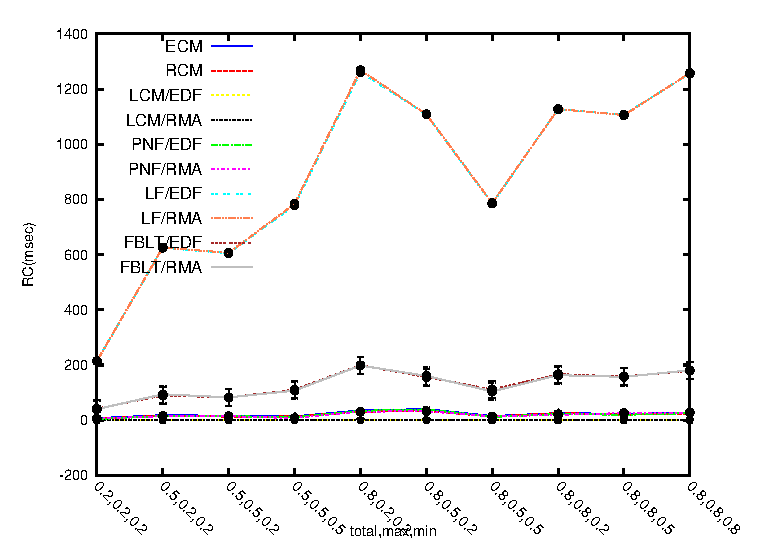
\includegraphics[scale=0.68]
{/e/lectures/real-time/PhD-work/STM/Practical/results_uno/figures/5_tasks/Abr_Dur/fblt/Abr_dur_5t_1obj_all_100wr}
\label{fig:fblt_results_1_obj_all}
}
%~
\subfigure[ECM, RCM, LCM, PNF, FBLT]{
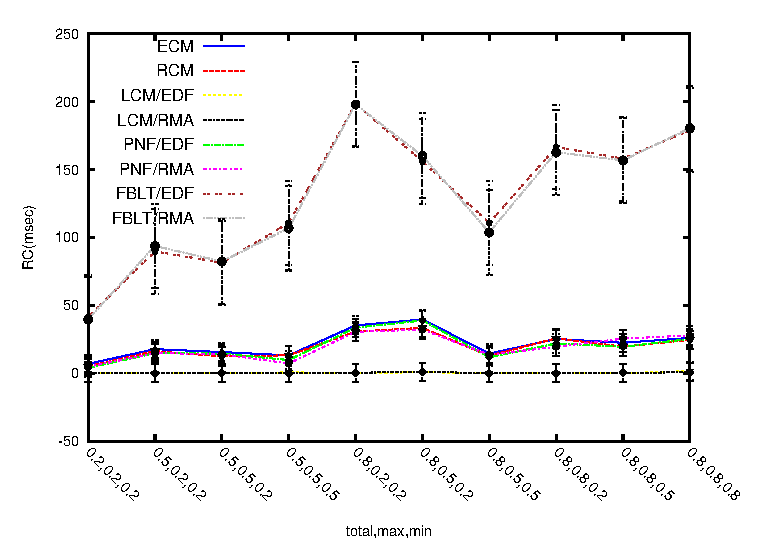
\includegraphics[scale=0.68]
{/e/lectures/real-time/PhD-work/STM/Practical/results_uno/figures/5_tasks/Abr_Dur/fblt/Abr_dur_5t_1obj_100wr}
\label{fig:fblt_results_1_obj_without_lock_free}
}
\caption{Avgerage retry cost (one object/transaction).}

\label{fig:fblt_results_uniobject}
\end{figure}
%
Figure~\ref{fig:fblt_results_uniobject} shows the average retry cost for the 5 task set sharing one object. On the x-axis of the figures, we record 3 parameters $x$, $y$, and $z$. $x$ is the ratio of the total length of all atomic sections of a task to the task WCET. $y$ is the ratio of the maximum length of any atomic section of a task to the task WCET. $z$ is the ratio of the minimum length of any atomic section of a task to the task WCET. The confidence level of all data points is 0.95. While Figure~\ref{fig:fblt_results_1_obj_all} includes all synchronization methods, Figure~\ref{fig:fblt_results_1_obj_without_lock_free} excludes lock-free. From these figures, we observe that lock-free has the largest retry cost, as it provides no conflict resolution. FBLT has the largest retry cost among CMs,  because transactions share only one object in this case. For multiple objects per transaction, 
%
%FBLT provides equal or shorter retry cost than LCM, as shown in Figures~\ref{fig-RC-fblt-4t-20obj} and~\ref{fig-RC-fblt-4t-40obj}. 
PNF has an advantage over FBLT. However, PNF requires a-priori knowledge of all objects accessed by each transaction, whereas FBLT does not. Consequently, retry cost under PNF is a little shorter than that under FBLT. 
%For 8 and 20 task sets, FBLT's retry cost is comparable to PNF's as shown in Figures~\ref{fig-RC-fblt-8t-20obj} to~\ref{fig-RC-fblt-20t-40obj}. 
Experiments show that FBLT's retry cost can be shorter than that under ECM, RCM, and LCM, and can be comparable to that of PNF's as shown in Figure~\ref{fig-RC-fblt-20t-40obj}. 
%
\begin{comment}
\begin{figure}
\centering
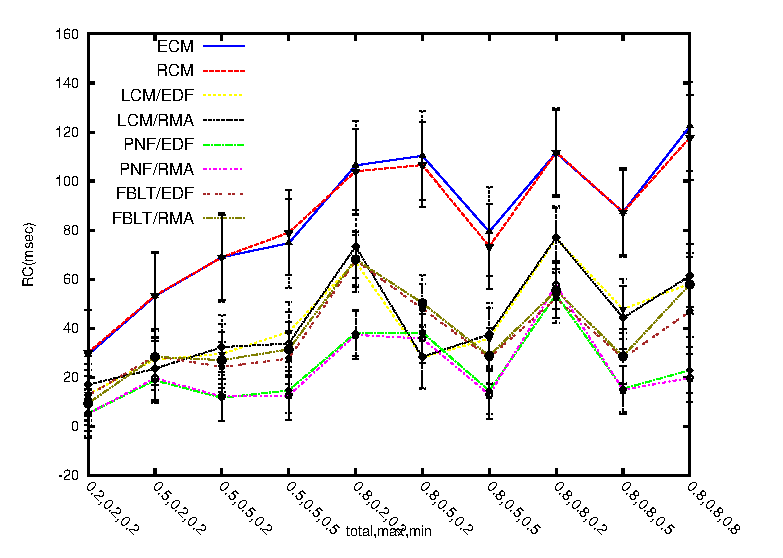
\includegraphics[scale=0.68]{/e/lectures/real-time/PhD-work/STM/Practical/results_uno/figures/4_tasks/Abr_Dur/fblt/Abr_dur_4t_50obj_100wr_-1eta}
\caption{Avgerage retry cost (20 shared objects, 4 tasks).}
\label{fig-RC-fblt-4t-20obj}%1
\end{figure}
%
\begin{figure}
\centering
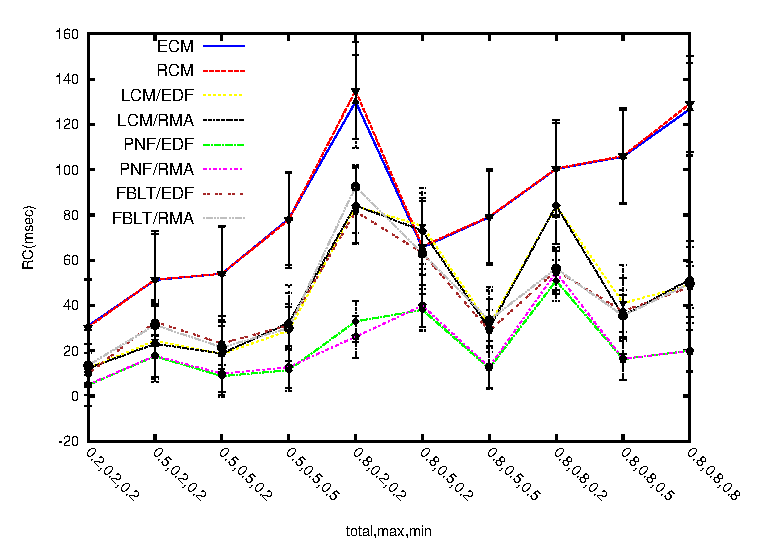
\includegraphics[scale=0.68]{/e/lectures/real-time/PhD-work/STM/Practical/results_uno/figures/4_tasks/Abr_Dur/fblt/Abr_dur_4t_100obj_100wr_-1eta}
\caption{Avgerage retry cost (40 shared objects, 4 tasks).}
\label{fig-RC-fblt-4t-40obj}
\end{figure}
%
\begin{figure}
\centering
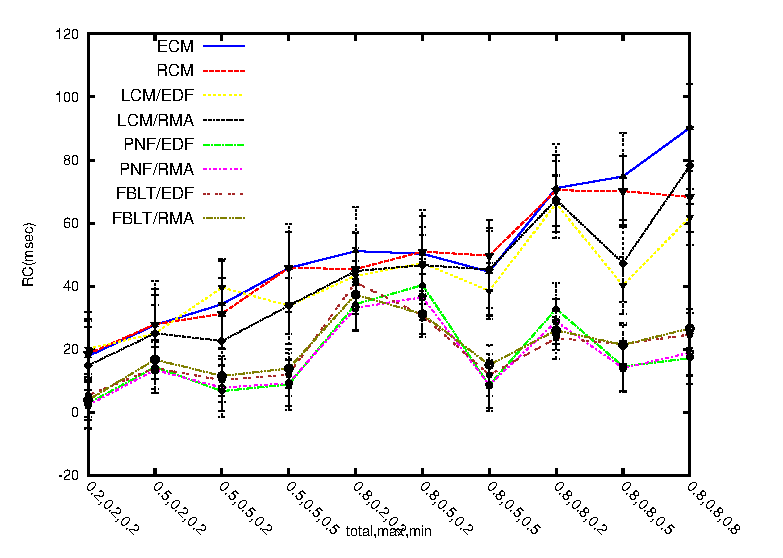
\includegraphics[scale=0.68]{/e/lectures/real-time/PhD-work/STM/Practical/results_uno/figures/8_tasks/Abr_Dur/fblt/Abr_dur_8t_90obj_100wr_-1eta}
\caption{Avgerage retry cost (20 shared objects, 8 tasks).}
\label{fig-RC-fblt-8t-20obj}
\end{figure}

\begin{figure}
\centering
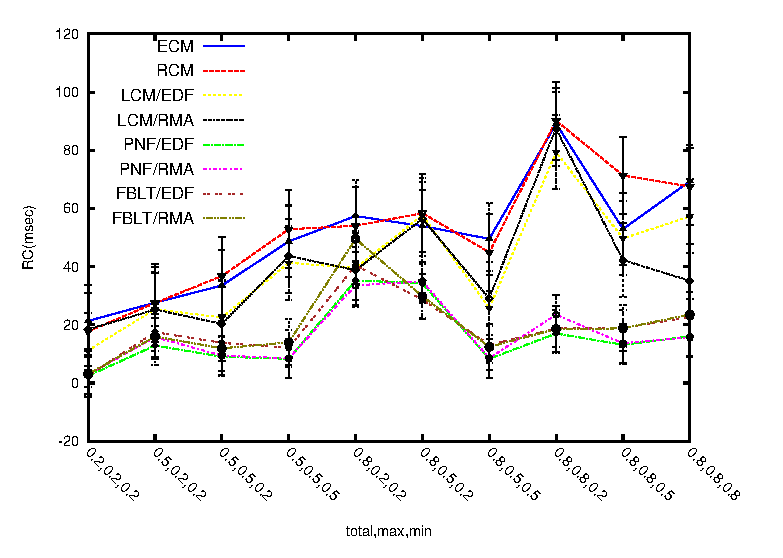
\includegraphics[scale=0.68]{/e/lectures/real-time/PhD-work/STM/Practical/results_uno/figures/8_tasks/Abr_Dur/fblt/Abr_dur_8t_180obj_100wr_-1eta}
\caption{Avgerage retry cost (40 shared objects, 8 tasks).}
\label{fig-RC-fblt-8t-40obj}
\end{figure}

\begin{figure}
\centering
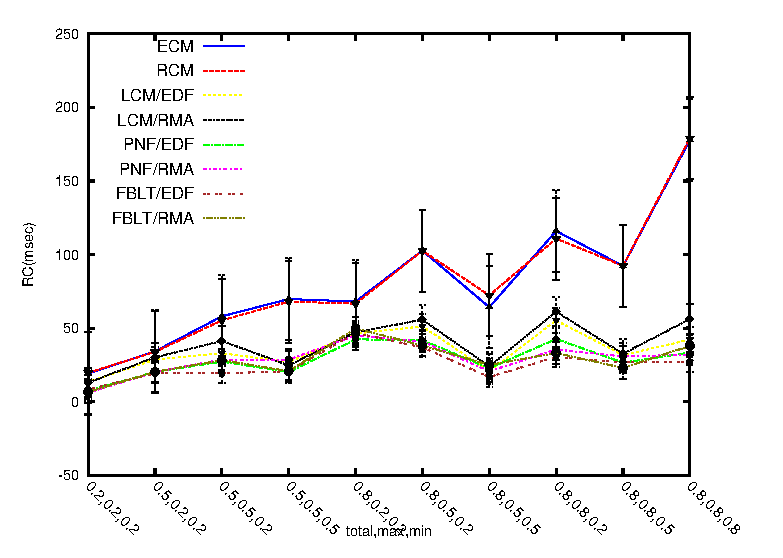
\includegraphics[scale=0.68]{/e/lectures/real-time/PhD-work/STM/Practical/results_uno/figures/20_tasks/Abr_Dur/fblt/Abr_dur_20t_210obj_100wr_-1eta}
\caption{Avgerage retry cost (20 shared objects, 20 tasks).}
\label{fig-RC-fblt-20t-20obj}
\end{figure}
\end{comment}
%
\begin{figure}
\centering
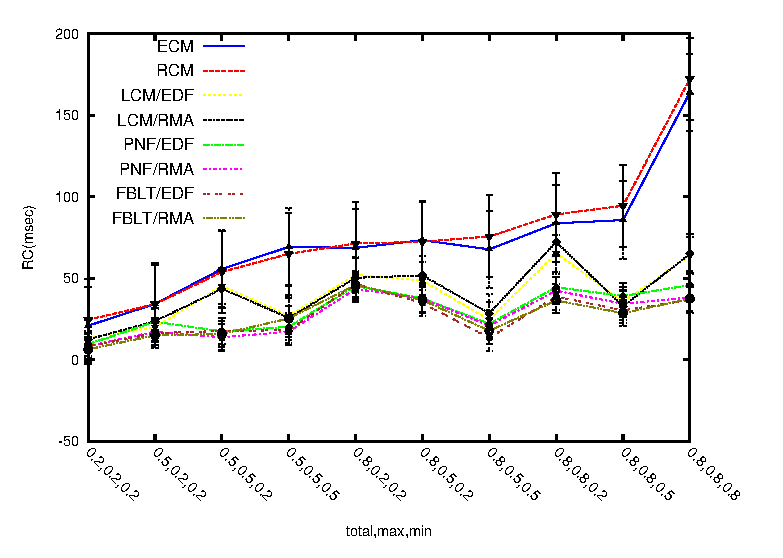
\includegraphics[scale=0.68]{/e/lectures/real-time/PhD-work/STM/Practical/results_uno/figures/20_tasks/Abr_Dur/fblt/Abr_dur_20t_420obj_100wr_-1eta}
\caption{Avgerage retry cost (40 shared objects, 20 tasks).}
\label{fig-RC-fblt-20t-40obj}
\end{figure}
%
PNF was designed to avoid transitive retry. Previous experiments compares retry cost of different CMs in case of transitive retry. Figure~\ref{fig-RC-fblt-4t-20obj_non_transitive} 
%to~\ref{fig-RC-fblt-20t-20obj_non_transitive} 
compares retry costs of different CMs in case of non-transitive retry. FBLT achieves shorter or comparable retry cost to other CMs including PNF. Similar trends were observed for the other task
sets; those are omitted here due to space limitations and available at~\cite{stmconcurrencycontrol_techreport}.
%
\begin{figure}
\centering
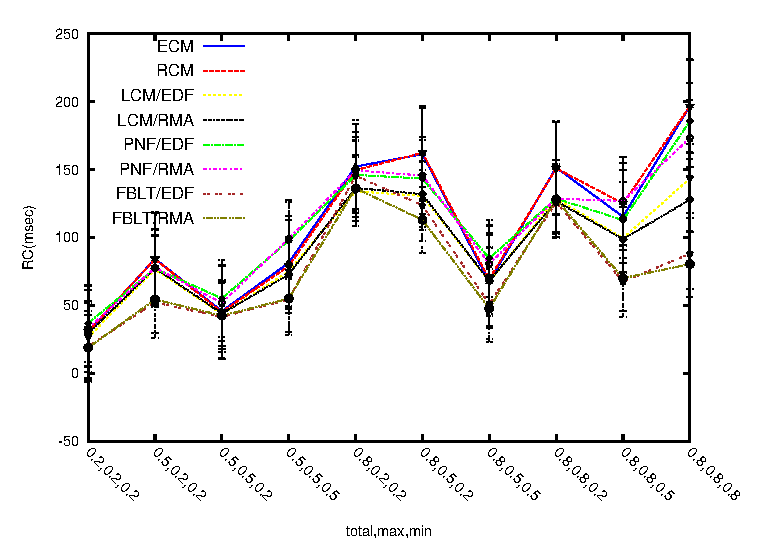
\includegraphics[scale=0.68]{/e/lectures/real-time/PhD-work/STM/Practical/results_uno/figures/4_tasks/Abr_Dur/fblt/Abr_dur_4t_20obj_100wr_-1eta}
\caption{Avgerage retry cost (20 shared objects, 4 tasks).}
\label{fig-RC-fblt-4t-20obj_non_transitive}
\end{figure}
%
\begin{comment}
\begin{figure}
\centering
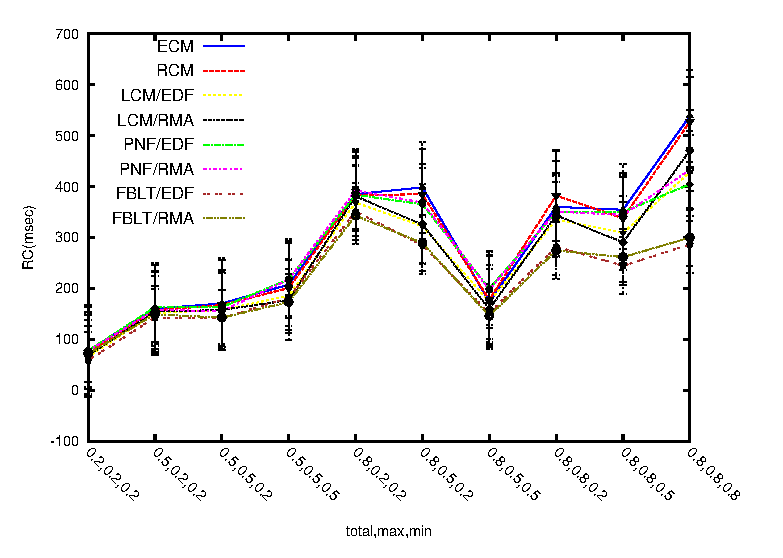
\includegraphics[scale=0.68]{/e/lectures/real-time/PhD-work/STM/Practical/results_uno/figures/8_tasks/Abr_Dur/fblt/Abr_dur_8t_20obj_100wr_-1eta}
\caption{Avgerage retry cost (20 shared objects, 8 tasks).}
\label{fig-RC-fblt-8t-20obj_non_transitive}
\end{figure}

\begin{figure}
\centering
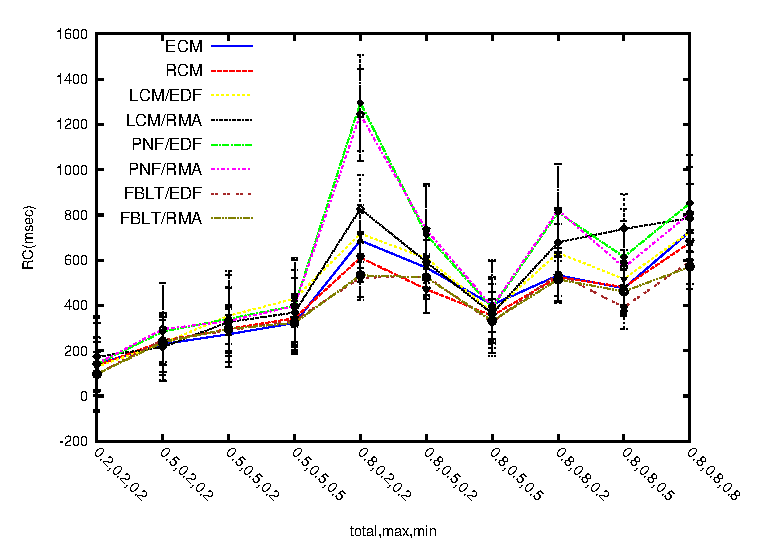
\includegraphics[scale=0.68]{/e/lectures/real-time/PhD-work/STM/Practical/results_uno/figures/20_tasks/Abr_Dur/fblt/Abr_dur_20t_20obj_100wr_-1eta}
\caption{Avgerage retry cost (20 shared objects, 20 tasks).}
\label{fig-RC-fblt-20t-20obj_non_transitive}
\end{figure}
\end{comment}


\section{Conclusions}\label{conclusion}

Transitive retry increases transactional retry costs under ECM, RCM, and LCM. PNF avoids transitive retry by avoiding transactional preemptions. It avoids transitive retry cost by concurrently executing non-conflicting transactions, which are non-preemptive. However, PNF requires a-priori knowledge about objects accessed by each transaction. This is incompatible with dynamic STM implementations. Thus, we introduce the FBLT contention manager. Under  FBLT, each transaction is allowed to abort for a no larger than a specified number of times. Afterwards, the transaction becomes non-preemptive. Non-preemptive transactions have higher priorities than other preemptive transactions and real-time jobs. Non-preemptive transactions resolve their conflicts using FIFO order. 
%
By proper adjustment of the maximum abort number of each transaction, we showed that FBLT's schedulability is equal to or better than PNF. 
%For FBLT's schedulability to be equal to or better than lock-free synchronization, the upper bound on $s_{max}/r_{max}$ must be 1. The upper bound on $s_{max}/r_{max}$ can be higher than 1 if transactions execute in their arrival order and contention is high. 
%
Our experimental results show that FBLT has equal or shorter retry cost than ECM, RCM, and LCM. PNF requires a-priori knowledge of all objects accessed by each transaction. This is an advantage for PNF over FBLT. Consequently, retry cost under PNF is shorter than that under FBLT in case of transitive retry. Still, FBLT's retry cost can be comparable to PNF's. In case of no or low transitive retry, FBLT achieves shorter retry cost than other CMs including PNF. 
%
Future work includes choosing another criterion to resolve conflicts of non-preemptive transactions. Also, using feedback from the system to adjust maximum abort number of each transaction. Consequently, retry cost can be reduced over time.

\bibliographystyle{IEEEtran}
\bibliography{IEEEabrv,global_bibliography}

\end{document}


